% Document class for LME theses: lmedoc
% %LANGUAGE
% %CONFIG
%    The option "german" uses german.sty
%    For english papers, use the "english" option
% Possible types of theses:
% bt - Bachelor's thesis
% mt - Master's thesis
% diss - Dissertation
% sa - Student thesis
% fp - Forschungspraktikum
% pa - Projektarbeit
%\documentclass[german,bt]{lmedoc/lmedoc}
\documentclass[english,bt]{lmedoc/lmedoc}
%\documentclass[english,fp]{lmedoc/lmedoc}


%%%%%%%%%%%%%%%%%%
% pdflatex and lualatex are supported
% ++ "Umlaut" support
%    The package "inputenc" can be used to write Umlaute or the german double s
%    directly. You need to use the correct encoding, e.g. latin1.
\usepackage{iftex}
\ifPDFTeX
  \usepackage[utf8]{inputenc}
  \usepackage[T1]{fontenc}
  \usepackage{lmodern}
\else
  \ifXeTeX
     \usepackage{fontspec}
  \else 
     \usepackage{luatextra}
  \fi
\fi

%Load additional packages
\usepackage{lmedoc/packages}
% put in this file your abbreviations
% add your abbreviations here
\newabbreviation{2d}{2D}{two-dimensional}
\newabbreviation{3d}{3D}{three-dimensional}

\newabbreviation{avit}{AViT}{Adapting Vision Transformer}

\newabbreviation{csa}{CSA}{Center Self-Attention}
\newabbreviation{cnn}{CNN}{Convolutional Neural Networks}
\newabbreviation{cpu}{CPU}{Central Processing Unit}
\newabbreviation{ct}{CT}{Computed Tomography}

\newabbreviation{efficientvit}{EfficientViT}{Efficient Vision Transformer}

\newabbreviation{fau}{FAU}{Friedrich-Alexander-Universität}
\newabbreviation{ffn}{FFN}{Feed-Forward Network}
\newabbreviation{fpn}{FPN}{Feature Pyramid Network}

\newabbreviation{id}{ID}{Identification}
\newabbreviation{iou}{IoU}{Intersection of Union}

\newabbreviation{gpu}{GPU}{Graphics Processing Unit}

\newabbreviation{k}{K}{Key}

\newabbreviation{lstm}{LSTM}{Long Short-Term Memory}

\newabbreviation{mhsa}{MHSA}{Multi-Head Self-Attention}
\newabbreviation{mhcsa}{MHSA}{Multi-Head Central Self-Attention}
\newabbreviation{miou}{mIoU}{mean Intersection of Union}
\newabbreviation{mlp}{MLP}{Multi-Layer Perceptron}
\newabbreviation{mvt}{MVT}{Mix-Vision Transformer}

\newabbreviation{nlp}{NLP}{Natural Language Processing}

\newabbreviation{pvt}{PVT}{Pyramid Vision Transformer}

\newabbreviation{q}{Q}{Query}

\newabbreviation{relu}{ReLU}{Rectified Linear Unit}
\newabbreviation{rnn}{RNN}{Recurrent Neural Network}

\newabbreviation{se}{SE}{Squeeze-and-Excitation}
\newabbreviation{shcsa}{SHCSA}{Single-Head Central Self-Attention}
\newabbreviation{shsa}{SHSA}{Single-Head Self-Attention}
\newabbreviation{shvit}{SHViT}{Single-Head Vision Transformer}
\newabbreviation{shvit_csa}{SHViT with CSA}{Single-Head Vision Transformer with Central Self-Attention}
\newabbreviation{simvit}{SimViT}{Simple Vision Transformer}
\newabbreviation{ssd}{SSD}{Solid-State-Drive}

\newabbreviation{tevit}{TeViT}{Temporally Efficient Vision Transformer}
\newabbreviation{unetr}{UNETR}{UNEt TRansformers}

\newabbreviation{v}{V}{Value}
\newabbreviation{vis}{VIS}{Video Instance Segmentation}
\newabbreviation{vit}{ViT}{Vision Transformer}

%%%%%%%%%%%%%%%%%%%%%%%%%%%%

% supress messages because of underful hbox, this is not a problem
\hbadness=10000

\usepackage[backend=biber]{biblatex}

% some useful commands
\makeatletter % let's define a single dot
\DeclareRobustCommand\onedot{\futurelet\@let@token\@onedot}
\newcommand{\@onedot}{\ifx\@let@token.\else.\null\fi\xspace}
\makeatother

\usepackage{float}
\usepackage{multirow}

\usepackage{threeparttable}
\newcommand{\CellWithForcedBreak}[2][c]{
	\begin{tabular}[#1]{@{}c@{}}#2\end{tabular}}

\usepackage[most]{tcolorbox}
\definecolor{dkgreen}{rgb}{0,0.6,0}
\definecolor{lightgray}{rgb}{0.95,0.95,0.95}
\definecolor{gray}{rgb}{0.5,0.5,0.5}
\definecolor{mauve}{rgb}{0.58,0,0.82}
\definecolor{red}{rgb}{0.8,0,0}

\lstnewenvironment{Python}
{
	\lstset{frame=tb,
		language=Python,
		aboveskip=3mm,
		belowskip=0mm,
		showstringspaces=false,
		columns=flexible,
		basicstyle={\small\ttfamily},
		%		numbers=left,
		%		stepnumber=1,
		%		numberstyle=\small\color{gray},
		keywordstyle=\color{blue},
		commentstyle=\color{dkgreen},
		stringstyle=\color{red},
		breaklines=true,
		breakatwhitespace=true,
		tabsize=3}}{}

\usepackage[autostyle=true]{csquotes}
\setquotestyle[guillemets]{german} %% erzeugt quotes wie: >> xxxxx <<


% Sets the bib file
\addbibresource{literature.bib}

% When writing a large document, it is sometimes useful to work on selected sections of the document.
% Use this command to only build the document partially. Speeds up the developement cycle.
% For the final product, this has to be commented out.
%\includeonly{introduction,appendix,foo,bar}


\pagenumbering{roman}

\begin{document}
\clearpage
% %CONFIG
% This is for students' theses
  \begin{deckblatt}
    \Titel{Evaluation of Single-Head Vision Transformer (SHViT) for Volumetric Semantic Segmentation in Industrial CT Scans} % Title
    \Name{Drewes} % Last name
    \Vorname{ChangGeng} % Given name
    \Matrikelnummer{22984031}
    \Geburtsort{Yokohama, Japan} % Place of birth
    \Geburtsdatum{16.02.2000} % Date of birth
    \Betreuer{Martin Leipert} % Advisor
    \Start{18.06.2025} % Start of thesis
    \Ende{18.08.2025} % End of thesis
    %\ZweitInstitut{ZweitInstitut} % Cooperation partner
  \end{deckblatt}


\cleardoublepage
% Only necessary for thesis

Ich versichere, dass ich die Arbeit ohne fremde Hilfe und ohne Benutzung
anderer als der angegebenen Quellen angefertigt habe und dass die Arbeit
in gleicher oder "ahnlicher Form noch keiner anderen Pr"ufungsbeh"orde
vorgelegen hat und von dieser als Teil einer Pr"ufungsleistung
angenommen wurde. Alle Ausf"uhrungen, die w"ortlich oder sinngem"a"s
"ubernommen wurden, sind als solche gekennzeichnet.
\\

\vspace{2cm}

\noindent ChangGeng Drewes

\cleardoublepage


\begin{center}
\bfseries
% Abstract in German
{\selectlanguage{german}"Ubersicht}
\normalfont
\end{center}

Diese Bachelorarbeit befasst sich mit der Anpassung und Erweiterung von 2D-Vision-Transformer-Modellen, insbesondere SegFormer mit Mix-Vision Transformer (MVT) und Single-Head Vision Transfomer (SHViT), für die volumetrische 3D-Segmentierung. Der Fokus liegt auf der präzisen Segmentierung von 3D-Schuhscans. Als zentrales Qualitätsmaß wurde die F1-Metrik verwendet.

\medskip 

Die Experimente zeigen, dass die Anzahl der Convolution-Layer im SHViT-Modell erheblichen Einfluss auf die Segmentierungsgenauigkeit und den GPU-Speicherverbrauch hat. Die beste Balance wurde mit zwei Convolution-Layern im PatchEmbed-Block erzielt. Um die Speicherbelastung durch klassische Attention-Mechanismen mit $O(n^2)$-Komplexität zu verringern, wurde ein Central Self-Attention-Ansatz auf Basis eines Sliding-Window-Verfahrens implementiert. Dieser reduziert den Speicherbedarf je nach Konfiguration um bis zu 54\%, ohne die Modellleistung wesentlich zu beeinträchtigen. Zusätzlich konnten kleinere Kernelgrößen im Attention-Block die Genauigkeit weiter steigern, da damit feine Strukturen besser erfasst werden können.

\medskip

Die besten Ergebnisse wurden mit einem SHViT-Modell mit Central Self-Attention und optimierter Parametrierung erzielt, bei dem der Speicherbedarf bei unter 24\,GB GPU-Speicherbedarf liegt. Abschließend wird angeregt, sich in zukünftigen Arbeiten weiter mit der Optimierung von Attention-Mechanismen zur Reduzierung des Speicherbedarfs zu befassen und weitere Vision-Transformer-Backbones zur Verbesserung der Segmentierungsgenauigkeit auszuprobieren.

\newpage

\begin{center}
\bfseries
% Abstract in English
{\selectlanguage{english}Abstract}
\normalfont
\end{center}

This bachelor’s thesis looks at how to improve and expand 2D Vision Transformer models, particularly SegFormer with Mix-Vision Transformer (MVT) and Single-Head Vision Transformer (SHViT), for 3D segmentation of volume data. The main emphasis is on accurately segmenting 3D shoe scans. The F1-metric was used as the primary performance measure.

\medskip

Experiments show that the number of convolutional layers in the SHViT model significantly affects both segmentation accuracy and GPU memory usage. The best trade-off was achieved with two convolutional layers in the PatchEmbed block. To mitigate the high memory demands of conventional attention mechanisms with $O(n^2)$ complexity, a central self-attention approach based on a sliding-window method was implemented. Depending on the configuration, this reduces memory requirements by up to 54\% without significantly affecting model performance. Furthermore, smaller kernel sizes in the attention block led to improved accuracy, as they allowed for better capture of fine structural details.

\medskip

The best results came from an SHViT model that used central self-attention (sliding windows) with improved backbone and decoder settings, while ensuring GPU memory use stayed under 24\,GB. Finally, the thesis recommends that future work should look into improving attention mechanisms to use less memory and examine other Vision Transformer backbones to improve segmentation accuracy.

\cleardoublepage

\begin{center}
	\bfseries
	% Abstract in English
	{\selectlanguage{english}Acknowledgments}
	\normalfont
\end{center}

I would like to express my gratitude toward everyone who supported me during my thesis project.

\medskip

First, I would like to thank my advisor, Martin Leipert, for giving me this interesting topic and the precious opportunity to do my bachelor's thesis in the Pattern Recognition Lab at Friedrich-Alexander-University. His mentorship and suggestions during this research project have been instrumental in shaping the direction and quality of my work. His encouragement and insightful advice have been a constant source of motivation and confidence. A special mention and heartfelt gratitude to Prof.~Dr.-Ing.~Maier for creating this opportunity, which allowed me to grow in the professional field. 

\medskip

Lastly, and most importantly, I thank my family for their constant support and encouragement. Without it, this assignment would not have been possible.

\medskip

Thank you all for making this thesis possible.

\bigskip

ChangGeng Drewes



\cleardoublepage

\tableofcontents

\cleardoublepage \pagenumbering{arabic}

\include{Introduction}   % Introduction 
\cleardoublepage
%\chapter{Literature Review}

\section{Overview of Transformer-Based Models}
Transformer-based models have revolutionized the field of artificial intelligence and machine learning, particularly in the domains of\gls{nlp} and computer vision. Initially introduced by Vaswani et al. in 2017 \cite{vaswani2023attentionneed}, transformers have rapidly become the architecture of choice due to their exceptional performance and flexibility.  In 2021, a research team at Google introduced the paper \enquote{An Image is Worth 16x16 Words: Transformers for Image Recognition at Scale} in 2021, which applied the Transformer encoder architecture to the image recognition (classification) task \cite{dosovitskiy2021imageworth16x16words}.

The transformer architecture is fundamentally different from previous sequence-to-sequence models like \glspl{rnn} and \gls{lstm} networks. It relies on an attention mechanism to process input data in parallel, rather than sequentially. This parallelization enables transformers to handle long-range dependencies more effectively and efficiently.

The key components of transformer models are:
\begin{itemize}
	\item Self-Attention Mechanism: Self-attention allows the model to weigh the importance of different words in a sentence relative to each other, capturing contextual relationships.
	\item Multi-Head Attention: This involves multiple attention layers (heads) that operate in parallel, enabling the model to focus on different parts of the input simultaneously.
	\item Positional Encoding: Because transformers do not inherently understand the order of sentences or words, positional encoding is used to inject information about the relative or absolute position of tokens in the sequence.
	\item Feedforward Neural Networks: Each transformer block contains a feedforward neural network that processes the attention outputs and introduces nonlinearity.
	\item Layer Normalization: Normalization layers stabilize and accelerate training by reducing internal covariate shift in the model.
\end{itemize}

For Vision Transformer the transformer architecture is extended to image data by dividing images into patches and processing them similarly to token sequences in \gls{nlp}.


\section{Image Segmentation}
Image segmentation is a critical task in the field of computer vision, aiming to partition an image into meaningful regions or segments, often corresponding to different objects or areas of interest. Unlike image classification, which assigns a single label to an entire image, segmentation seeks to label each pixel, providing a more granular understanding of the visual content.

There are several types of image segmentation, each serving a different purpose:
\begin{itemize}
	\item Semantic Segmentation: This involves classifying each pixel in the image into a class without distinguishing between different instances of the same class. For example, all pixels belonging to 'cars' will be labeled as 'car', regardless of the number of cars present.
	\item Instance Segmentation: This not only classifies each pixel but also distinguishes between different instances of the same class. For example, each car in an image will be individually labeled.
	\item Panoptic Segmentation: This combines both semantic and instance segmentation, providing a complete scene understanding by labeling all pixels and distinguishing different instances.
\end{itemize}

Evaluating the performance of segmentation models involves several metrics, including:
\begin{itemize}
	\item \gls{iou} or Jaccard index, which is the ratio of the intersection area to the union area of the predicted ($A$) and ground truth segments ($B$): 
	\begin{equation}
		\text{IoU} = \frac{\left| A \cap B \right|}{\left| A \cup B \right|} = \frac{\left| A \cap B \right|}{\left| A \right| + \left| B \right| - \left| A \cap B \right|}
	\end{equation}
	The Jaccard Distance Loss is the defined as: 
	\begin{equation}
		\text{Jaccard-Distance-Loss} = 1 - \text{IoU}
	\end{equation} If there is no intersection between the two classes $A$ and $B$, then $\left| A \cap B \right| = 0$ and $\text{IoU}=0$ and $\text{Jaccard-Distance-Loss} = 1$. In an experiment with multiple segmentations \gls{iou}  is averaged over all single \glspl{iou}: 
	\begin{equation}
		\text{IoU} = \frac{1}{N} \sum_{i=1}^N \text{IoU}_i
	\end{equation}
	\item Dice Coefficient: Similar to \gls{iou} but gives more weight to correctly predicted areas, particularly useful for dealing with imbalanced datasets. 
	\item Pixel Accuracy: The ratio of correctly classified pixels to the total number of pixels. However, for imbalanced data this metric shouldn't be used.
\end{itemize}

Modern segmentation models, such as \gls{shvit} and Segformer, leverage transformer architectures to enhance model performance and flexibility. These models integrate self-attention mechanisms to capture global context and fine-grained details, pushing the boundaries of segmentation quality and efficiency.


\section{Segformer: Architecture, Applications, and Performance}
Segformer is a state-of-the-art image segmentation model that leverages the power of transformers to achieve high-performance on various segmentation tasks. Introduced by researchers at NVIDIA, Segformer addresses the limitations of conventional \glspl{cnn} and transformer-based models by combining their strengths to provide an efficient and scalable solution for image segmentation.

Segformer adopts a unique architecture that integrates the advantages of transformers with the computational efficiency of \glspl{cnn}. The model comprises two main components:
\begin{itemize}
	\item Hierarchical Transformer Encoder: The encoder uses hierarchical transformers to capture multi-scale contextual information from the input image. Unlike traditional vision transformers that process image patches of a fixed size, Segformer employs a hierarchical structure to progressively reduce the spatial resolution while increasing the receptive field. This allows the model to capture fine-grained details at higher resolutions and global context at lower resolutions.
	
	\item Lightweight All-MLP Decoder: The decoder in Segformer is built using multi-layer perceptrons (MLPs) instead of convolutional layers. This lightweight design reduces computational complexity and makes the model more efficient. The decoder aggregates the multi-scale features extracted by the encoder and generates dense segmentation maps.
\end{itemize}



\section{SHViT: Architecture, Applications, and Performance}

\section{Analysis of 2D and 3D Modeling Techniques}

\section{Comparative Analysis of SHViT and Segformer}

\section{Summary}
   % (\chapter{})
%\cleardoublepage

\include{Methodology}   % (\chapter{})
\cleardoublepage


\chapter{Data Preparation} \label{data_preparation}
Before starting to develop and train a machine learning model, it is important to examine the dataset at hand. In this first step, the dataset must be checked in detail to learn how it is structured, what types of data it contains and whether the data is consistent and reliable. This in‑depth exploration is essential, as the data's quality and structure affect the model's performance and prediction validity.


\section{Detailed Analysis of the Dataset}
By analyzing the dataset, inconsistencies, missing values, or anomalies that could potentially distort the results can be identified. In addition, this process helps to understand the relationships between different variables, ensures that the data is representative of the problem area, and can provide accurate and meaningful insights.


\subsection{Shoe Dataset Acquisition Using Computed Tomography}
The shoe dataset used in this thesis is the same as used in a previous study, the results of which were presented in a conference paper \cite{contribution_martin_leipert}. 40 high-resolution \gls{3d} scans of shoes in boxes are created using a Werth Tomoscope operating at 200\,kV. The scans produced high-resolution volumetric data with a voxel size of 340\,µm and volumes approximately $1000^3$ voxels in size. Each scan captured not only the shoe structure but also the surrounding packaging materials (e.g., cardboard boxes and stuffing paper). 

\medskip

To generate training data for the segmentation, the \gls{ct} volumes were manually labeled using \gls{3d} Slicer \cite{Fedorov_Slicer3D}. The process involved annotating each boxed shoe pair in three stages, corresponding to the segmentation steps. Seed points are placed in regions representing the shoe, packaging material, and background. These seed points are gradually expanded, followed by manual corrections near boundaries where shoe and packaging overlapped. The shoe was further segmented into outer sole, insole, and upper material based on differences in \gls{ct} density and structure. The outer sole, being dense and thick, was easily distinguishable, and the insole appeared as a softer layer above it, while the upper was thinner and more variable in material. The labeling process of each shoe pair took up to three hours, depending on their complexity. The authors note that the labeled dataset contains some minor misclassification errors, mostly due to boundary ambiguities and labeling complexity. These are assumed to be random and are addressed during training \cite{contribution_martin_leipert}.

\medskip

Each \gls{3d} shoe scan is saved in {\tt.rek}-format\footnote{Before the data can be extracted from the file, the Python package {\tt PythonTools-3.7.0-py2.py3-none-any.whl} must be installed manually.}, with file sizes ranging from 500\,MB to almost 5\,GB, and is intended to represent the input data for the segmentation model to be created. The corresponding ground-truth dataset with annotated segmentation labels are compressed and saved in a proprietary file format {\tt .seg.nrrd}\footnote{NRRD stands for \enquote{Nearly Raw Raster Data} \url{https://pynrrd.readthedocs.io/en/stable/background/about.html}} designed for efficient storage and retrieval and the file sizes ranges from 13\,MB to nearly 160\,MB.


\subsection{Visualisation of 3D-Dataset} \label{sec::visualizing_the_volumes}
The first step in analyzing the dataset involves visualizing the \gls{3d} dataset to gain a clearer understanding of its structure and contents. Hence, a Python program was written to process and visualize the data. 

\medskip

The libraries {\tt rek2py} and {\tt slicerio}\footnote{\url{https://pypi.org/project/slicerio/}} are used to extract the data of the scan dataset with {\tt .rek} file format and the annotated segmentation data of the ground-truth {\tt .seg.nrrd} files. All \gls{3d}-scan files in the folder were read in individually with the script, their data extracted into header and volume with the {\tt rek2py} function, the volume data then was split into slices, and saved. The sizes of the volume data ranges from {\tt (958, 410, 685)} up to {\tt (1056, 1071, 1068)}, which also correlates quite well with the file sizes. 

\medskip

During analysis of the individual images, it became evident that image quality varied significantly. This inconsistency was mainly caused by brightness scaling across the entire volume, likely due to different \gls{ct} scan settings. Such variability posed challenges for consistent preprocessing and model input normalization. To address this, the concept of histogram stretching was applied: the minimum and maximum percentiles were set to 1\% and 99\%, respectively, based on trial and error, in order to enhance the contrast and brightness of the image. This approach helped reduce the influence of outliers and improve visual consistency across the dataset. Based on these percentile thresholds, the corresponding minimum and maximum intensity values for each shoe were calculated using the NumPy function {\tt np.percentile()}. These values were then needed to scale and clip the entire volume to the range {\tt [0,1]}. An exception was made for the shoe {\tt PetrolioSch-40-float\_down2\_2\_2}, where the lower percentile threshold had to be set to 4\%.

\medskip

The example plot of two views of a \gls{3d} shoe scan (figure \ref{Bruschi_down2_2_2_3d}) shows the full volume on the left, while the image on the right displays a cross-sectional cut through the scan. 

\begin{figure}[H]
	\centering
	\begin{minipage}{.5\textwidth}
		\centering
		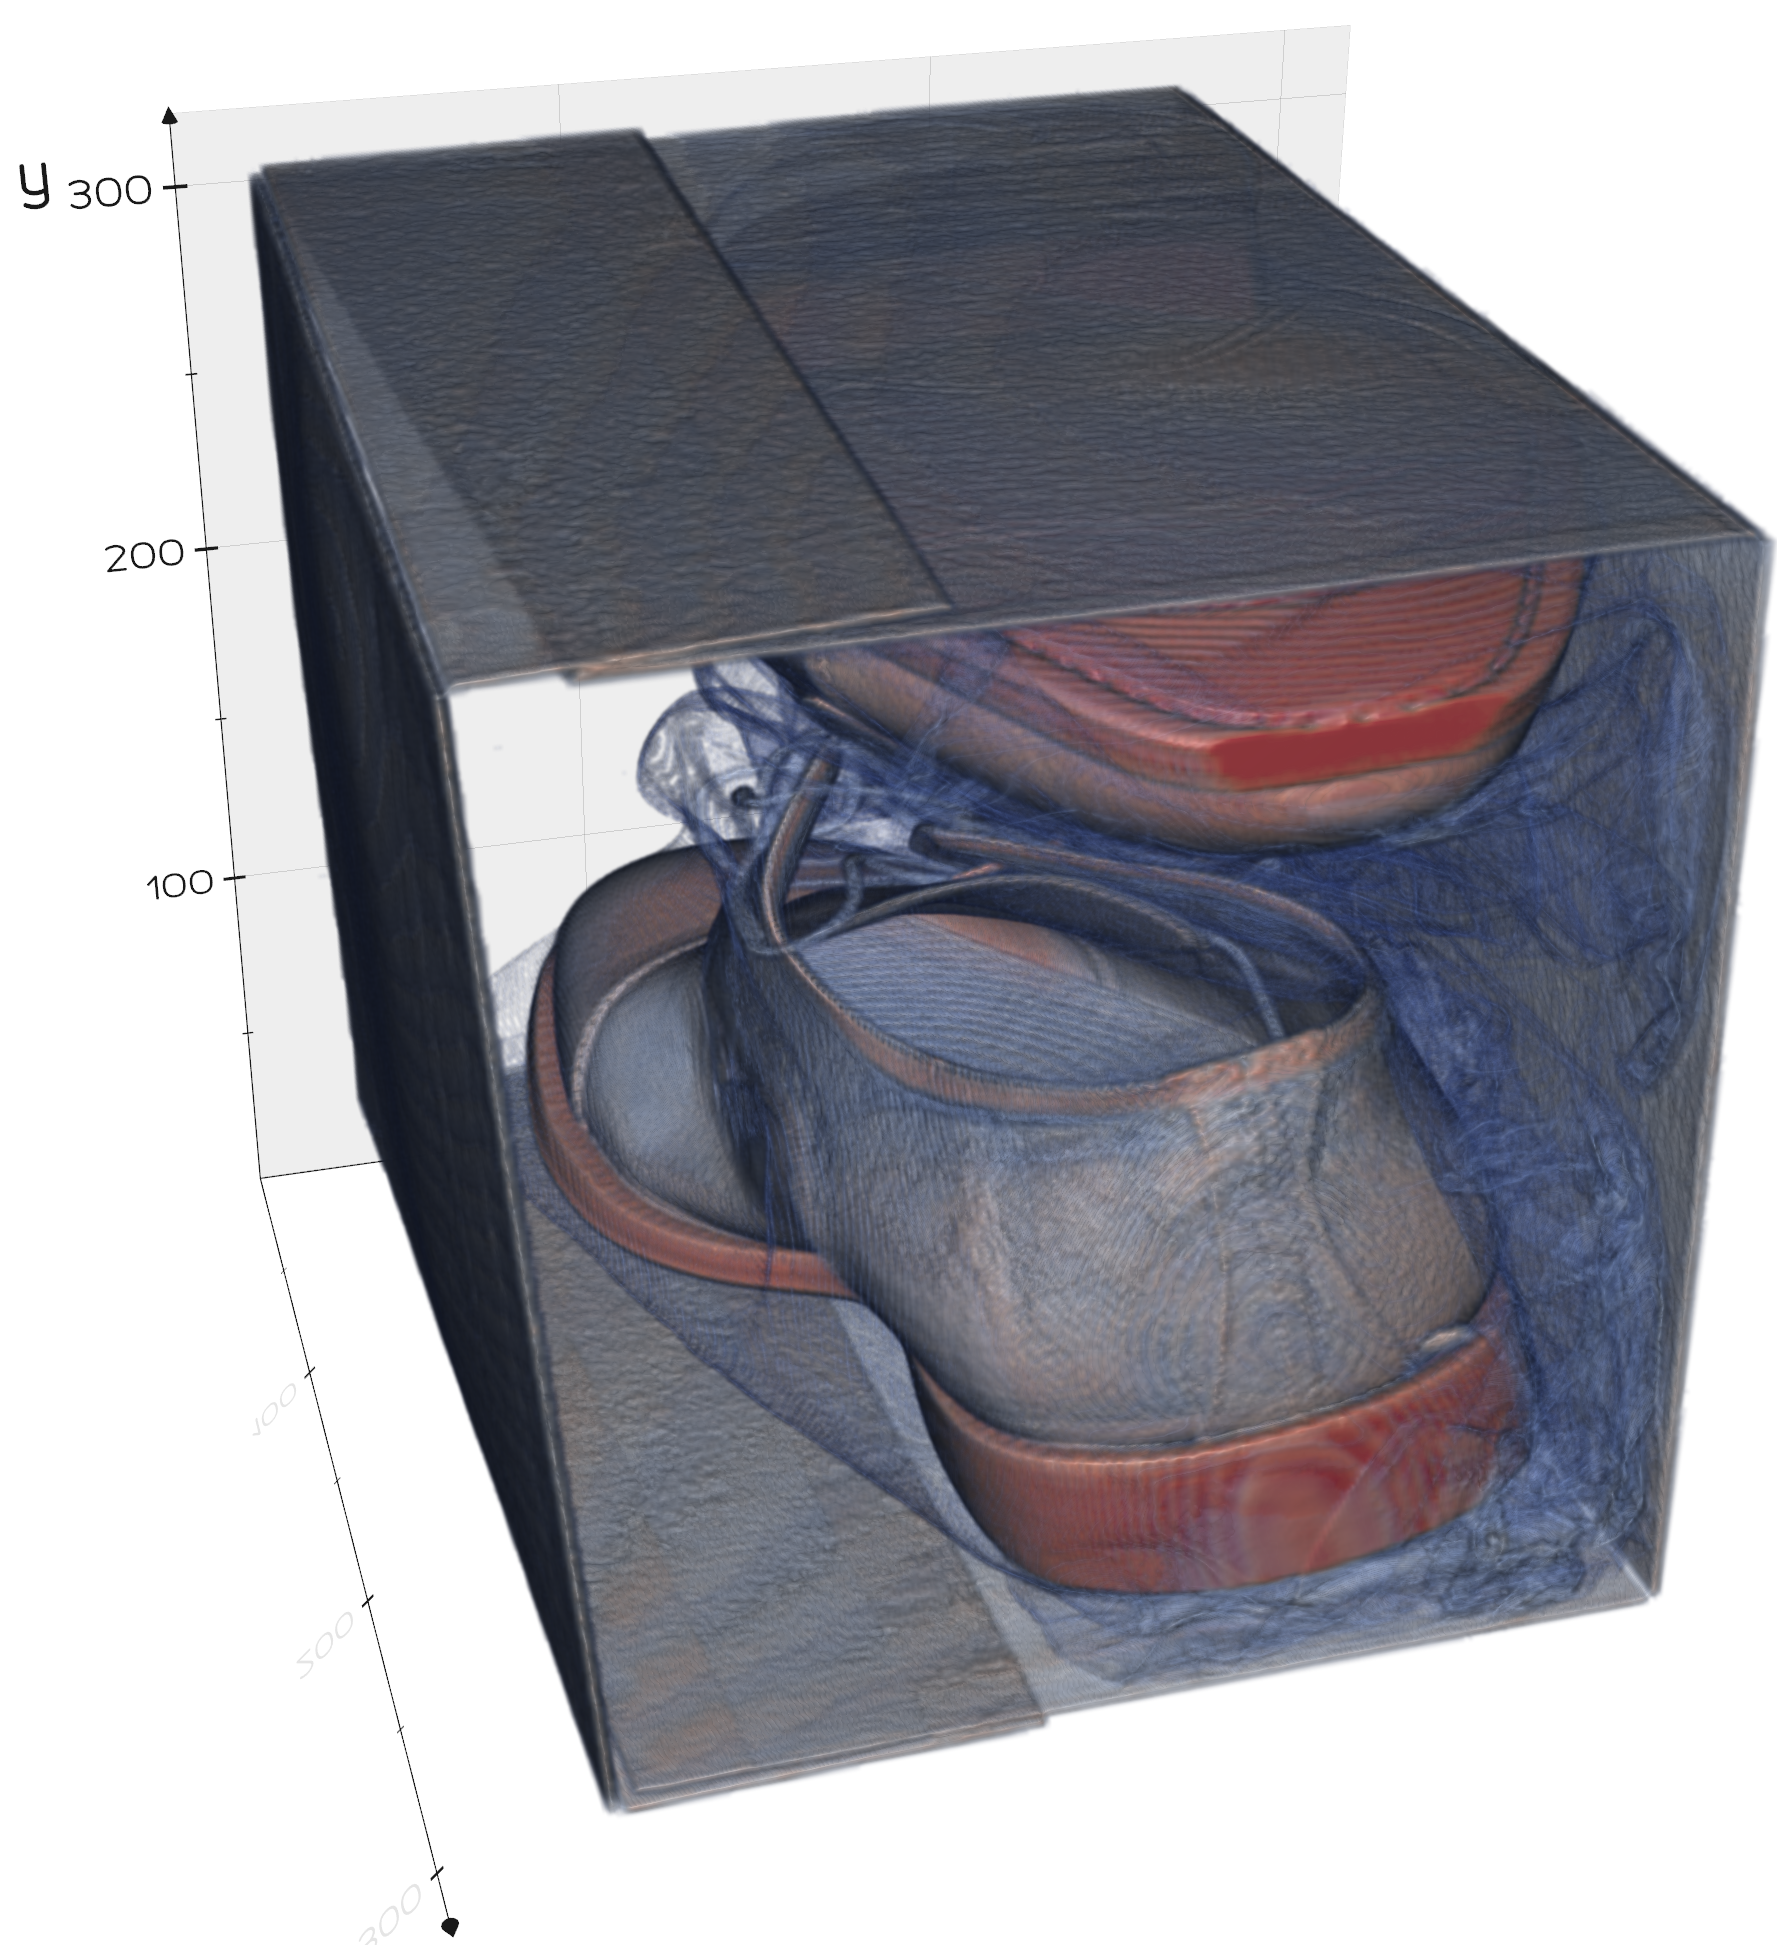
\includegraphics[width=1.0\textwidth]{./images/Bruschi_down2_2_2_3d.png}
	\end{minipage}%
	\begin{minipage}{.5\textwidth}
		\centering
		\centering
		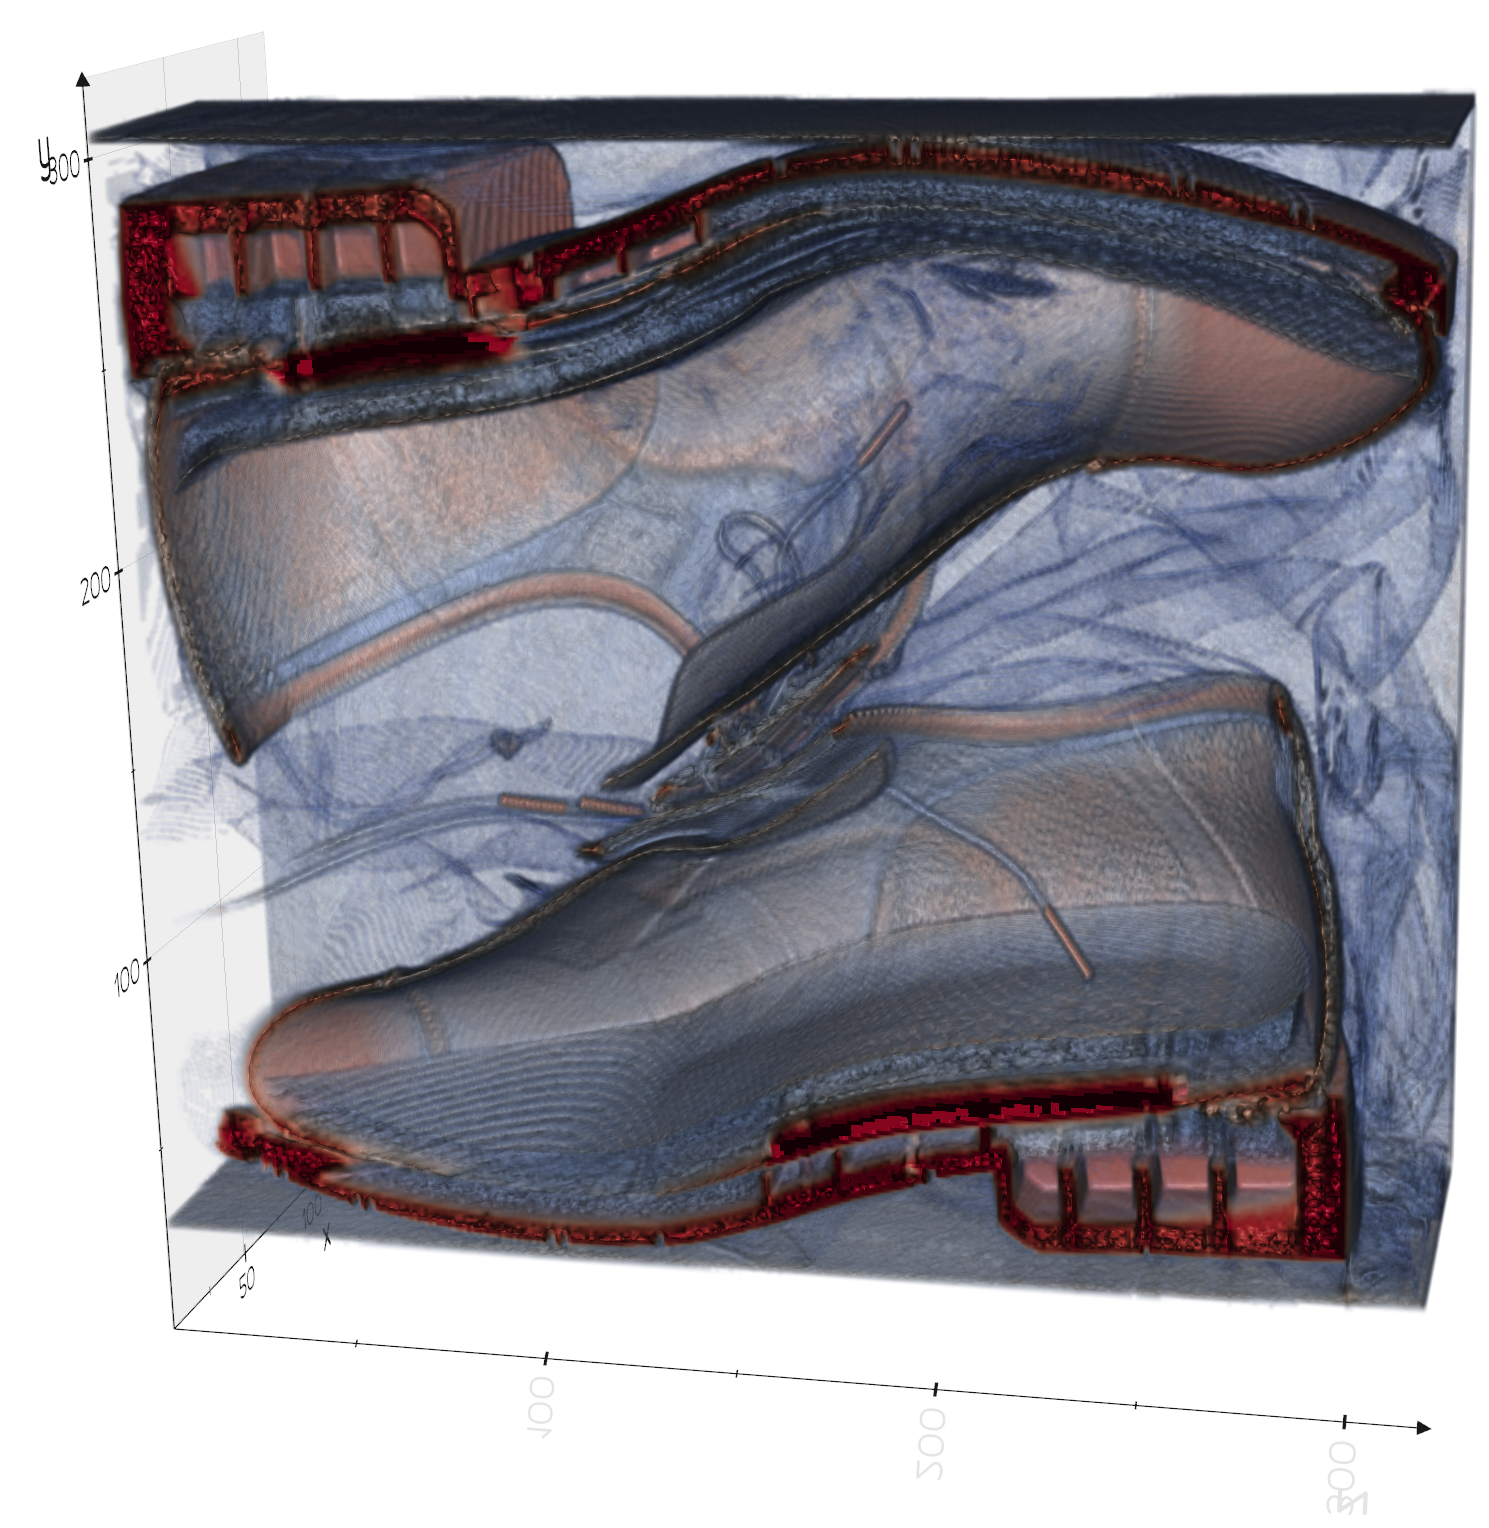
\includegraphics[width=1.0\textwidth]{./images/Bruschi_down2_2_2_3d_half.png}
	\end{minipage}
	\caption[3D-scan of {\tt Bruschi\_down2\_2\_2.rek}]{3D-scan of {\tt Bruschi\_down2\_2\_2.rek} with the original resolution of {\tt (876,650,475)} downsampled to {\tt (320,320,320)}.}
	\label{Bruschi_down2_2_2_3d}
\end{figure}

Another display variant consists of a series of slices taken from the scan. Figure \ref{Bruschi_down2_2_2} shows 24 cross-sections of the same shoe. In these images, the pair of shoes inside the box is visible and the soles, upper materials, box, and packing materials are clearly distinguishable.
\begin{figure}[H]
	\centering
	\includegraphics[width=1.0\textwidth]{./images/Bruschi_down2_2_2.png}
	\caption[File {\tt Bruschi\_down2\_2\_2.rek} with the resolution {\tt (876, 650, 475)}]{File {\tt Bruschi\_down2\_2\_2.rek} with the resolution {\tt (876, 650, 475)}. Shown are 24 different layers representing the third dimension.}
	\label{Bruschi_down2_2_2}
\end{figure}

When retrieving the associated segmentation plots for the file {\tt Bruschi\_down2\_2\_2}, the 12 segment names are {\tt Background}, {\tt Schuh\_1}, {\tt Schuh\_2}, {\tt Karton}, {\tt Innenvolumen\_1}, {\tt Innenvolumen\_2}, {\tt Ober\-material}, {\tt Innensohle}, {\tt Au(ß)ensohle}\footnote{When extracting the labels, the German umlauts and the 'ß' character are not displayed.}, {\tt F(ü)llmaterial}, {\tt Zunge}, {\tt Dummyschuh}. The label {\tt Dummyschuh} was originally introduced as a temporary helper class to combine the masks of both shoes into a single segment. However, this label was never actually used in the training or evaluation pipeline and is therefore not relevant for the segmentation task. Its presence in a few files results from it not being fully removed during preprocessing.

\medskip

Due to inconsistencies in the ordering of labels across annotation files, labels were not assigned based on index positions. Instead, each segment was identified and assigned according to its label name to ensure correctness regardless of order. This approach ensured that label mappings remained robust even when annotation files differed in structure or completeness.

\medskip

Only the six segments {\tt Karton}, {\tt Außensohle}, {\tt Innensohle}, {\tt Obermaterial}, {\tt Zunge}, and {\tt Füllmaterial} are used as ground-truth labels for the segmentation for the training of the model. The original {\tt Background} image provided in the dataset could not be used because it was incorrect. It should highlight only regions that do not belong to any of the shoe or packaging components. However, the original version contained inconsistencies; for example, some parts of the shoes were marked as background. Therefore, a new background mask was created by inverting the sum of the six segments mentioned above. The background, as shown in figure~\ref{Bruschi_down2_2_2_Segmentation}, is now correct.

\begin{figure}[H]
	\centering
	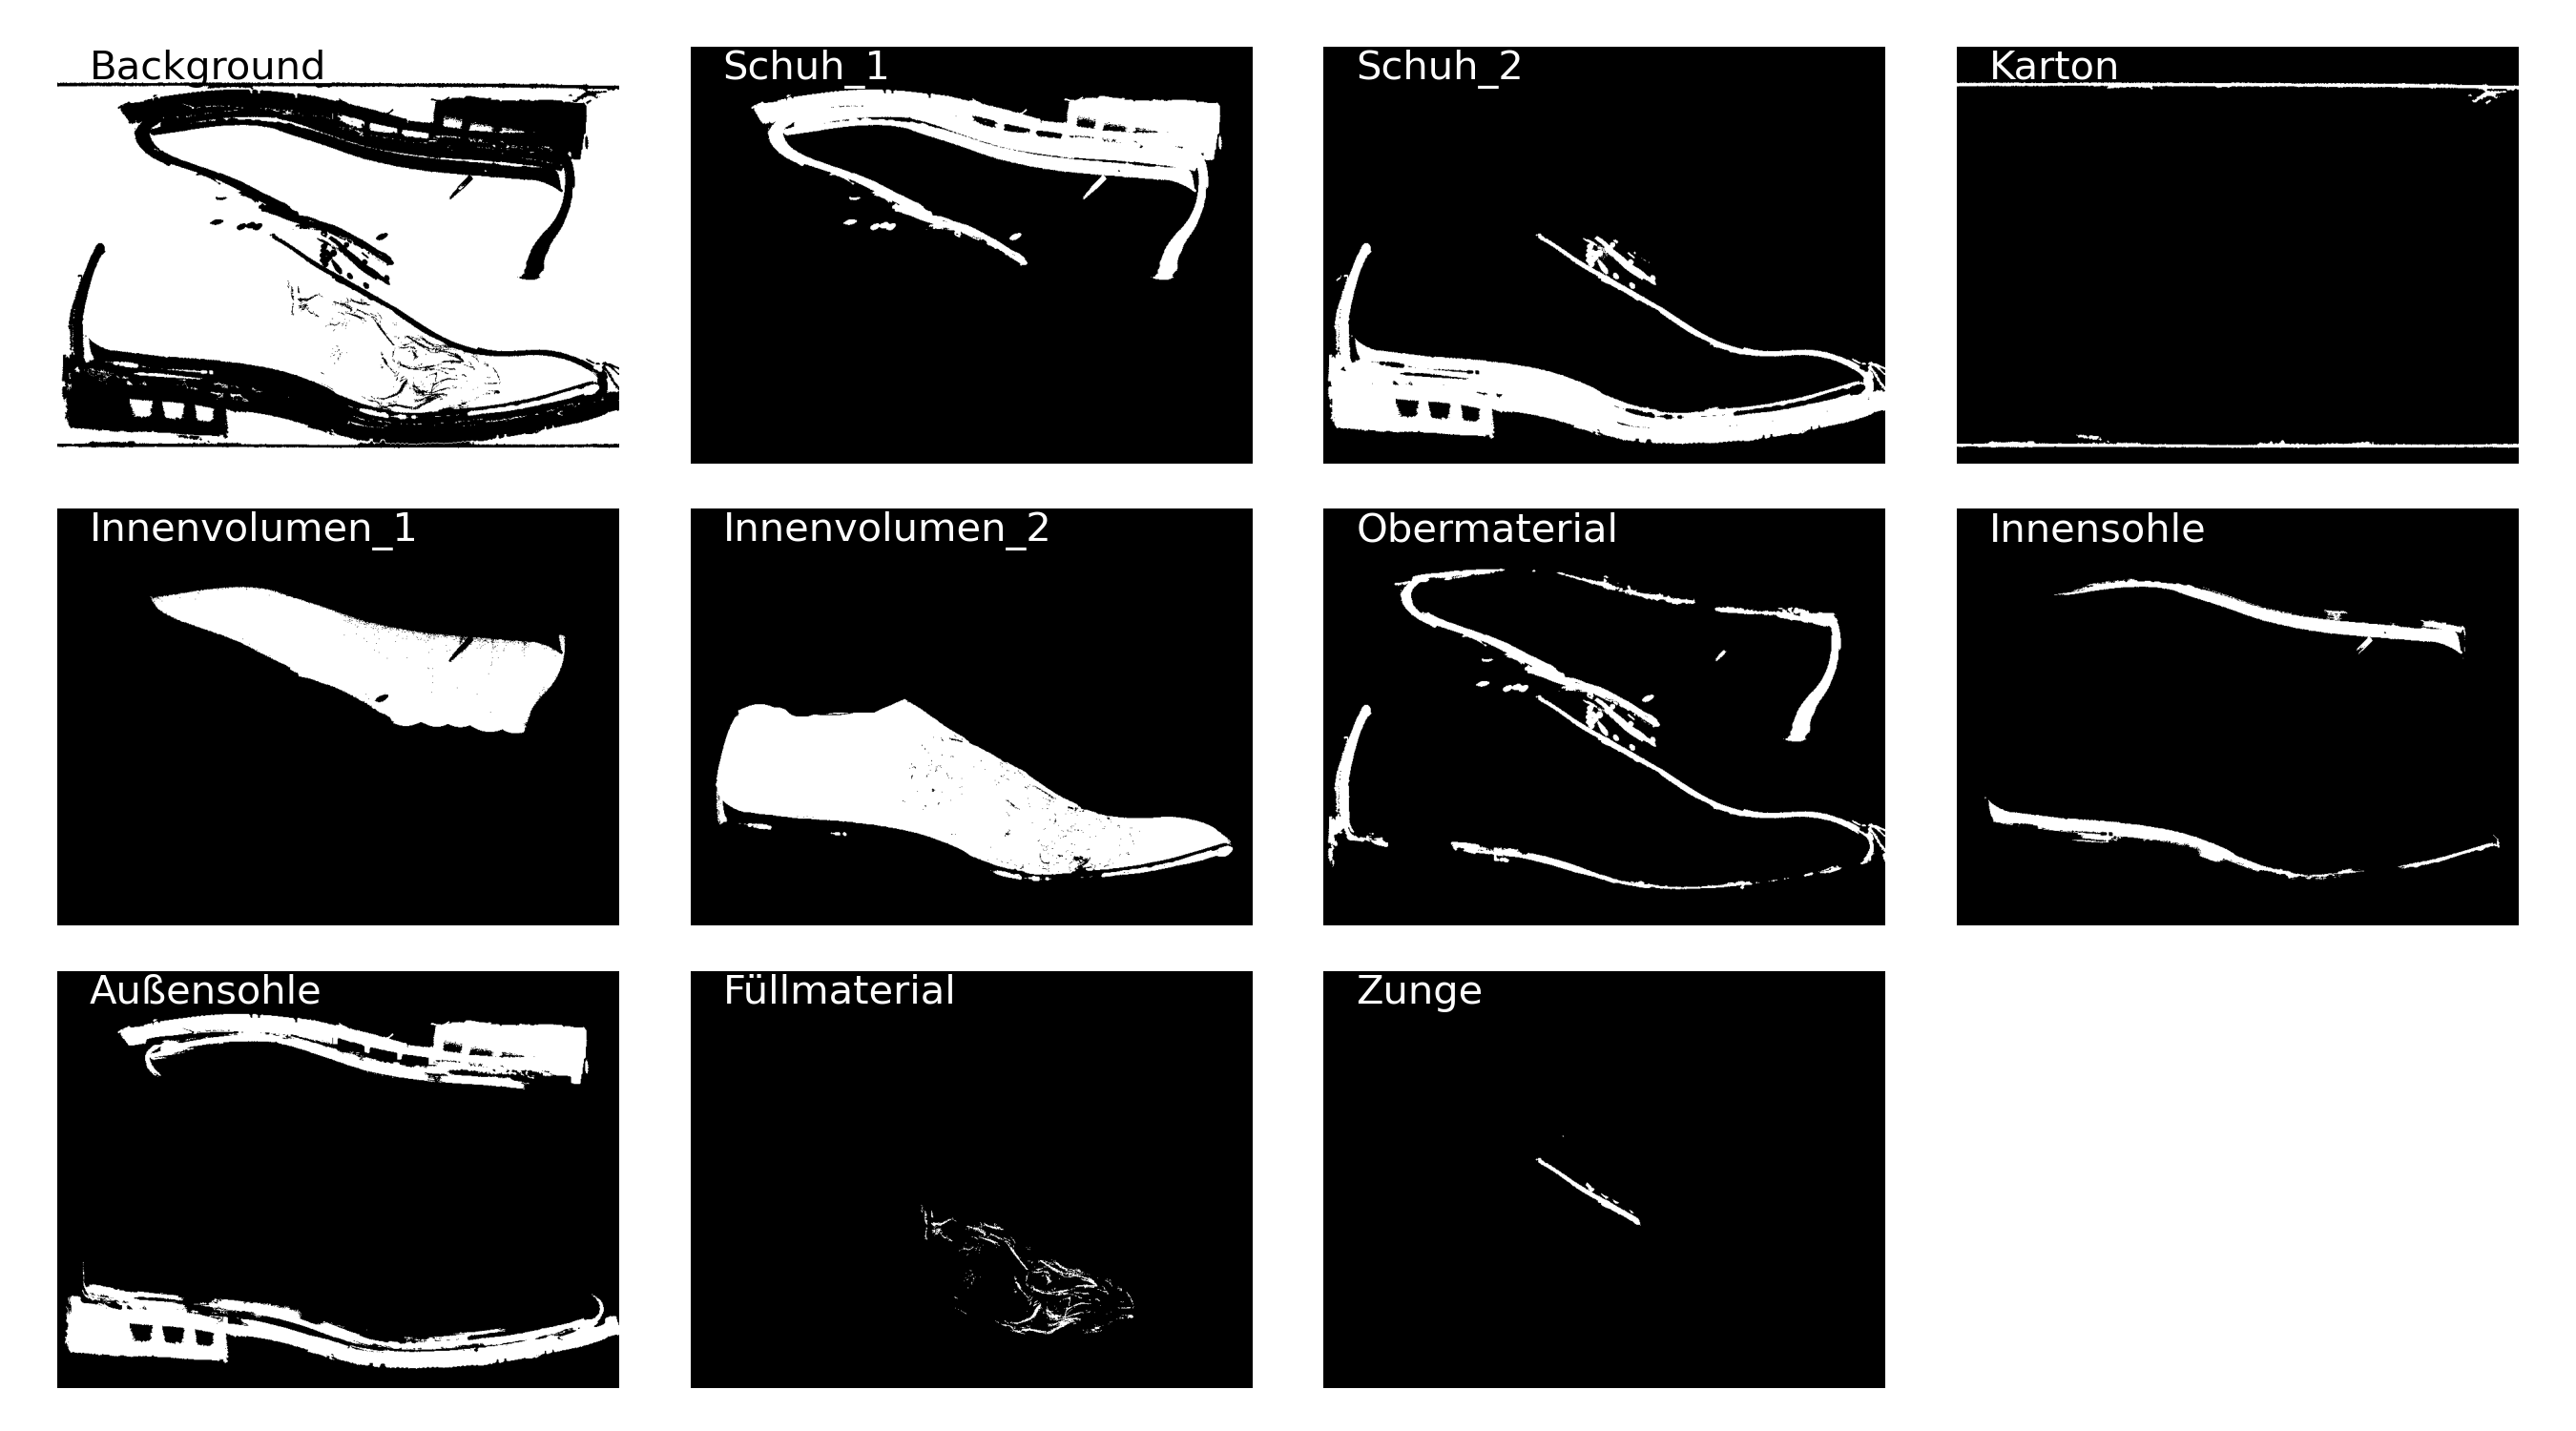
\includegraphics[width=1.0\textwidth]{./images/Layer_335_v2.png}
	\caption[Visualisation of all 11 segments for annotation file {\tt Bruschi\_down2\_2\_2}]{Visualisation of 11 segments for annotation file {\tt Bruschi\_down2\_2\_2.seg.nrrd}, Layer: 335}
	\label{Bruschi_down2_2_2_Segmentation}
\end{figure}

For the segmentation of the \gls{2d} images, a representative layer was selected by hand for each shoe somewhere in the middle of the \gls{3d} data set. The orientation for seven pair of shoe scans was also adjusted so that they can be seen in the sectional plane from the side. The shoe images were saved under the file name of the {\tt rek} file, and the seven label or segment images under the name of the annotation file. The image/segment files are assigned via key-value pairs in a dictionary. 

\medskip

The preprocessing step involves generating input volumes that are scaled to a cubic shape with dimensions depth (D) $\times$ height (H) $\times$ width (W), whereby depth, height, and width was set to be equal.  The segmentation file is then created by downscaling this volume by a factor of $2^N$ where $N$ is the number of {\tt Conv2d} or {\tt Conv3d} layers used in the overlay patch embedding module of the model head (see also figure \ref{Architecture_of_SHViT}). The downsampled segmentation volume also retains equal dimensions across all three axes. For example, if the input volume has dimensions {\tt (224, 224, 224)} and the overlay patch embedding contains two {\tt Conv3d} layers, the resulting segmentation files will have dimensions {\tt (56, 56, 56)}, due to the cumulative downscaling factor of $2^2=4$.



\section{Data Augmentation used for Training}
Data augmentation is essential when training deep learning models on small datasets. Given the limited availability of only 40 volumetric shoe scans, the network faces a significant risk of overfitting and reduced generalization \cite{HaoDataAugmentation}. Augmentation of the training set with transformed copies of each volume artificially expands the dataset and better approximates the true data distribution. Segmentation tasks in particular usually rely heavily on both the quantity and the quality of ground truth data and annotation of \gls{3d} volumes is very costly \cite{SutassananonDataAugmentation}. To avoid this, augmentation techniques that apply geometric transforms to the \gls{3d} volumes are commonly deployed. More generally, surveys of segmentation on small datasets emphasize that \enquote{data augmentation techniques are of great importance} because collecting sufficient volumetric annotations is \enquote{notoriously difficult} \cite{AlomarDataAugmentation}.

\medskip

In addition to the limited number of labeled volumes, recent studies emphasize the relationship between model complexity and required dataset size. Alwosheel et al.~\cite{ALWOSHEEL2018167} suggest that, to achieve stable generalization and avoid overfitting, the number of training samples should be at least ten times the number of trainable parameters. Given that the segmentation model used in this work contains approximately 13.8 million trainable parameters, and each \gls{3d} scan provides approximately 11.2 million voxels\footnote{Each volume has a resolution of {\tt (224,224,224)}, resulting in roughly 11.2 million voxels. If each voxel is seen as an independent training sample, at least ten volumes would be required to match the 1:10 data-to-parameter ratio for the \gls{shvit_csa} model. However, because of strong spatial correlations between neighboring voxels in semantic segmentation, the effective number of independent samples per scan is actually lower than it might appear. As a result, substantially more shoe volumes are needed, potentially 10 to 50 times more, depending on model complexity and data redundancy, as discussed in \cite{ALWOSHEEL2018167}.}, neither a single volume nor ten volumes provide a sufficient number of independent training samples. This further underlines the importance of applying targeted data augmentation to synthetically increase both the size and variability of the dataset.

\medskip

Data augmentation should be matched to the nature of the dataset, ideally reflecting its intrinsic variations. In the case of the shoe dataset, only horizontal flipping and $90^\circ$ rotations were applied, as these transformations align with the realistic orientations found in the scanned volumes. Shoes are generally placed in a consistent and orderly manner within the boxes, rather than in random or chaotic positions. Additionally, variations in brightness were observed, caused by fluctuations in exposure time that differ between individual \gls{ct} scans.

\medskip

To increase the diversity of the shoe-volume dataset, several standard volumetric augmentation methods are applied. In \gls{3d} space, simple affine transformations can generate new views of each shoe without altering its shape. In addition to geometric transformations, adjustments to brightness and contrast are also employed to simulate variations in scan conditions and improve model robustness. Commonly used operations include \cite{HaoDataAugmentation, AlomarDataAugmentation, SutassananonDataAugmentation}:
\begin{itemize}
	\item Axis-aligned flips (mirroring): Reflecting the volume across one of its principal planes (e.g. sagittal, coronal or axial) produces a mirror image of the shoe. This is equivalent to swapping one coordinate axis (for example flipping left-right across the sagittal plane). Flips preserve all voxel neighborhoods and create a valid alternative orientation. In practice, mirroring along each axis can roughly double or triple the dataset size (depending on symmetry).
	
	\item $90^\circ$ Orthogonal rotations: Rotating the entire \gls{3d} volume by $90^\circ$, $180^\circ$, or $270^\circ$ about any of the three coordinate axes creates new views. For instance, turning the shoe scan by $90^\circ$ around the vertical (z) axis creates a different front-back orientation, while a $90^\circ$ rotation about the left-right (x) axis tilts the shoe forward. By applying rotations in $90^\circ$ increments it is ensured that voxel values remain aligned on the grid (no interpolation artifacts) and the shoe's shape is preserved.
	
	\item Combined transforms: These basic flips and rotations can be composed to create additional variations. For example, a shoe volume might first be flipped left–right and then rotated $180^\circ$ about the vertical axis, resulting in a novel viewpoint. Each combination still preserves the shoe geometry while presenting it differently.
	
	\item To make the system more reliable under different \gls{ct} imaging conditions, the brightness and contrast of the voxel intensities are increased. Brightness augmentation means adding a small value to all voxel numbers to mimic changes in exposure levels. In contrast, contrast augmentation rescales voxel intensities relative to the mean, thereby enhancing or diminishing the distinction between dense and less dense regions. These transformations preserve the structural integrity and spatial relationships within the volume while enabling the network to generalize more effectively to scans acquired under different imaging settings or with varying material compositions. For the augmentation, brightness values are randomly selected from the set {\tt [-0.2, -0.1, 0.0, 0.1, 0.2]}, and contrast factors from {\tt [0.8, 0.9, 1.0, 1.1, 1.2, 1.3]}. Given the \gls{3d} volume \enquote{vol}, the following formulas are applied:
	\begin{align}
		\text{vol} &= (\text{vol} - 0.5) \cdot \text{contrast} + 0.5 \\
		\text{vol} &= \text{vol} + \text{brightness}
	\end{align}
	After applying these transformations, voxel intensities are clipped to the range {\tt [0,1]} to maintain valid intensity values.
\end{itemize}

Each of these augmentations produces a new training example. When applied to all 40 original scans, the effective training set grows by a factor equal to the number of distinct transforms used. Importantly, because these are rigid-body transformations, the ground-truth segmentation masks can be identically transformed (flipped or rotated) to match the augmented volumes. This guarantees label consistency because the shoe and its segmentations rotate together. 

\medskip

This method of increasing the size of volumetric datasets is well documented and has been proven to enhance segmentation accuracy in similar medical imaging problems \cite{HaoDataAugmentation, AlomarDataAugmentation, SutassananonDataAugmentation}. By applying these augmentations, the model can better generalize from only 40 original scans to the full variability of real-world shoe orientations and \gls{ct} imaging conditions, such as differences in brightness and contrast.

\medskip

While data augmentation is a practical and effective strategy to reduce overfitting, recent findings suggest that modern deep neural networks are capable of generalizing well even on small, noisy datasets. Olson et al.~\cite{NEURIPS2018_fface838} demonstrated that large neural networks can achieve strong performance on datasets with only a few hundred training examples, without necessarily overfitting. Their analysis shows that overparameterized networks behave like ensembles of low-bias, weakly correlated sub-networks, which introduces an implicit regularization effect. This supports the rationale for applying deep learning models even in small-data settings, especially when combined with targeted augmentation strategies that reflect the domain-specific structure of the data.

\medskip

There is no contradiction between the importance of data augmentation for small \gls{3d} segmentation datasets and the findings of Olson et al. Instead, both perspectives are complementary: data augmentation helps mitigate the high cost and limited availability of annotated volumetric data, while the study by Olson et al.~demonstrates that modern deep neural networks are capable of generalizing well, even when trained on small datasets \cite{NEURIPS2018_fface838}. This is particularly relevant when combined with suitable augmentation strategies. Together, these approaches enable effective training of deep models in scenarios where large-scale labeled data is not available.


\section{Implementation Details}
Before training, all input data undergo a structured preprocessing pipeline to ensure consistency and compatibility with the segmentation model. The preprocessing procedure consists of two main stages: processing the volumetric image data and preparing the corresponding annotation files.

\medskip

In the first stage, each shoe scan, which is stored as a \gls{3d} volume, is loaded from disk. To establish a uniform viewpoint across the dataset, some of the volumes are rotated such that all shoes are viewed consistently from the side. Following this orientation correction, all volumes are resized to a common cubic shape, meaning that the height, width, and depth of each volume are scaled to the same fixed value. This same resizing guarantees that all inputs have identical dimensions, which is particularly important when working with \gls{3d} convolutional neural networks, as it simplifies the design of the model and ensures spatial uniformity. After resizing, brightness normalization is applied as described in section \ref{sec::visualizing_the_volumes}, where pixel intensity values are scaled and clipped based on fixed percentile thresholds. The preprocessed volumes are then saved in NumPy format for downstream processing with only one \enquote{color} channel.

\medskip

In the second stage, the corresponding annotation files are handled. Each annotation file contains a full voxel-wise segmentation map in which multiple segments or labels are defined (see also section \ref{sec::visualizing_the_volumes}). For the purposes of this work, only seven (including background) specific labels are retained. These selected segments represent the most structurally and semantically relevant parts of the shoe. The segmentation volumes are then rotated using the same transformation applied to the associated shoe volume to preserve alignment. Next, the label volumes are resized according to the spatial resolution required by the segmentation head of the network, taking into account the number of convolutional layers and their respective downsampling effects.

\medskip

Finally, the segmentation labels are stored in a single \gls{3d} NumPy array per shoe, where voxel values range from 0 (background) to 6, with each integer value uniquely representing one of the seven selected shoe segments. This compact and standardized format ensures efficient loading during training and allows for direct compatibility with loss functions that expect integer-coded segmentation masks.

\bigskip

This study implemented the standard SegFormer with \gls{mvt} and \gls{shvit} backbones using PyTorch. TensorFlow was initially considered for the implementation. However, a memory leak was observed during its use, with the available \gls{gpu} memory gradually decreasing over time. This issue has been documented in TensorFlow's GitHub issues and has persisted without resolution\footnote{\url{https://github.com/tensorflow/tensorflow/issues/61791}}. Notably, it is present since TensorFlow v2.11 but was not seen in v2.9. To mitigate this issue, the TensorFlow code of SegFormer was ported to PyTorch, which offers more transparent memory management and enhanced control over resource allocation.
\gls{shvit} was already coded in PyTorch, thus requiring only minor adjustments to harmonize the interfaces for \gls{mvt} and \gls{shvit}.

\medskip

Furthermore, the code initially developed for \gls{2d} applications was restructured to also process \gls{3d} volumetric scans. A notable enhancement was the integration of the sliding-window attention mechanism, elaborated upon in the preceding section (see section \ref{Transformer_Attention_Mechanisms}). The original source code, taken from the \gls{simvit} GitHub repository\footnote{\url{https://github.com/ucasligang/SimViT/blob/main/classification/simvit.py}}, underwent slight modifications. Notably, the Python scripts are designed to function without installing additional libraries, such as {\tt timm}\footnote{\url{https://pypi.org/project/timm/}}, which is often used.

\medskip

To allow experiments with \gls{shvit} focusing on variables such as kernel size and the use or omission of central self-attention, additional modifications were made to the initialization routines of the respective classes. Details of the entire code are available in appendix \ref{sec::shvid_3d.py}, on pages \pageref{sec::shvid_3d.py}ff.

\medskip

The {\tt \_\_init\_\_} functions of the two SegFormer models, {\tt SegFormer3D} (with \gls{mvt}) and {\tt SegFormer3D\_SHViT}, were designed to accept the same input parameters, even if some were not used universally. This approach allows the models to be easily interchanged without requiring modifications to the model invocation in the main program.

\medskip

The main program used for training is a Jupyter notebook file. In this file, the model is loaded, and the data loaders are initialized for training, validation, and test datasets with augmentation. Additionally, the functions for the F1-score metric and -loss are defined. The program includes callbacks for warm-up, early-stopping, logging, and saving model parameters if improvements in the validation metrics occur.

\medskip

The training function begins with a warm-up phase reserved for the initial 20 epochs, during which the learning rate gradually increases to its target value. Following the warm-up, the actual training process starts, utilizing gradient accumulation with  {\tt BATCH\_SIZE=1} and {\tt ACCUMULATION\_STEPS=5}. After the data loader is applied to the training data, validation is conducted using the validation dataset to evaluate F1-score and -loss.

\medskip

Although data augmentation techniques are used to artificially expand the dataset, the underlying diversity remains limited to the original 40 shoe-samples. Cross-validation ensures that the models's ability to generalize is tested across different subsets of the original base shoes because normal train-test-splits can result in insufficient data for either training or validation purposes. Cross-validation, with {\tt kFold=5} in this thesis, addresses this limitation by utilizing every sample for both training and validation across different folds, thereby maximizing the informational value extracted from available data. It is important that the same original image does not appear in both training and validation sets within the same fold \cite{Kohavi_1995, Arlot_Celisse_2010}. Known as \enquote{data leakage prevention}, this principle maintains the independence between training and test data, and it is fundamental to get unbiased performance estimates\footnote{see also section 2.4 of \cite{Kapoor_Narayanan_2023}}. 

\medskip

At the end of each epoch, the F1-score and -loss values for both training and validation are displayed. If no improvement in validation F1 is observed within a specified number of epochs, the learning rate is reduced and the internal counter is reset, and training continues. Should the metric still fail to improve within another set of epochs, early stopping is triggered and training is terminated.

\medskip

Finally, curves for F1-score and -losses during training and validation are plotted. The best model, determined by the lowest validation loss, is loaded and used with the test dataset. All input images or volumes are loaded, segmentation predictions are generated, and the results are visualized by comparing the original input, the predicted segmentation, and the ground truth.
   % (\chapter{})
\cleardoublepage
\chapter{Experimental Setup, and Evaluation Results}\label{Results_and_Discussion}
In this chapter, the experiments and results of the training and evaluation of the \gls{3d} shoe scan segmentation models are presented. Several experiments were conducted to analyze the performance and efficiency of different network configurations. The baseline model is the standard SegFormer architecture, which uses an \gls{mvt} as backbone. This model is compared against two alternative configurations: SegFormer with \gls{shvit} as backbone, and a modified version of SHViT: \gls{shvit_csa} that incorporates a central self-attention mechanism designed to improve spatial focus but also reduces memory consumption.

\medskip

\noindent The experiments are structured into five main parts:
\begin{enumerate}
	\item Backbone comparison: SegFormer with \gls{mvt}, \gls{shvit}, and \gls{shvit_csa} backbones are compared under various parameter settings. Model performance is evaluated using the F1-score as the primary accuracy metric, and \acrshort{gpu} memory consumption is reported to assess computational efficiency.
	
	\item Volume test: The maximum input volume size that can be processed by the \gls{shvit}-based model under hardware constraints is determined, revealing useful information about their scalability.
	
	\item Convolution layer depth: The number of convolutional layers in the \gls{shvit} head is varied, and its impact on segmentation performance (in terms of F1 but also voxel resolution) is analyzed.
	
	\item Kernel size analysis: The effect of varying kernel sizes in both the central self-attention mechanism and the attention block of the \gls{shvit} model is investigated to understand their influence on model accuracy.
	
	\item Direct comparison with literature: The segmentation performance of the proposed \gls{shvit}-based model is compared against existing approaches with \glspl{cnn} in the literature \cite{contribution_martin_leipert}. The evaluation focuses on benchmark metrics, particularly the F1-score for each segmented component on the same dataset, offering both qualitative and quantitative insights into how \gls{shvit} performs relative to \gls{cnn}-based methods.
\end{enumerate}

Together, these experiments aim to provide a comprehensive evaluation of transformer-based architectures for \gls{3d} volumetric segmentation of shoe scans, highlighting trade-offs between model complexity, accuracy, and computational requirements.

\medskip

For each configuration in the experiment, six independent training runs were performed to account for variability due to random initialization and data augmentation. From these six simulations, the best five (based on validation performance) were selected. The final reported F1-score for each configuration is the average of these five values. Error bars in the plots in the following sections represent the standard deviation across these best five runs, providing a measure of the model's stability and robustness.



\section[Backbone Comparison: MVT, SHViT, and SHViT with CSA]{Backbone Comparison: SegFormers with MVT, SHViT, and SHViT with Central Self-Attention}
The first experiment focuses on evaluating the impact of different backbone architectures on the segmentation performance of \gls{3d} shoe scans. As a baseline, the standard SegFormer model with an \gls{mvt} backbone is used. This backbone has shown strong performance in \gls{2d} semantic segmentation tasks \cite{xie2021segformersimpleefficientdesign} and serves as a reference point for comparison.

\medskip

To explore more efficient and potentially better-suited alternatives for volumetric data, the \gls{mvt} backbone is replaced with \gls{shvit}, which is designed to better capture spatial dependencies in \gls{3d} data while maintaining computational efficiency. Furthermore, a modified version of \gls{shvit} is introduced, in which the conventional self-attention mechanism is replaced with a central self-attention block. This modification aims to enhance local spatial sensitivity and improve segmentation quality, particularly in regions with fine-grained structural details, but also helps to reduce memory consumption.

\medskip

All models in this experiment use a fixed input volume size of {\tt (224,224,224)} voxels and a segmentation output size of {\tt (56,56,56)}, determined by the number of downsampling steps and convolutional layers. Specifically, a two-layer convolutional encoder head is used across all configurations to map the feature representations to the final segmentation mask. Larger volumes such as {\tt (256,256,256)} exceed the available \acrshort{gpu} memory of 24\,GB when using the \gls{shvit} backbone with the B5/S4 configuration, and a fair comparison would not be possible.

\medskip

Each of these backbone configurations is tested using various hyperparameter settings to assess their robustness and performance under different conditions. The models are evaluated based on their segmentation accuracy, measured using the F1, their \acrshort{gpu} memory consumption, and the number of trainable parameters. This comparison illustrates the trade-offs between model complexity, resource requirements, and segmentation quality when applying transformer-based architectures to \gls{3d} imaging data.

\bigskip

Figure \ref{iou_vs_gpu_memory} shows a plot of F1-score versus \acrshort{gpu} memory consumption for the different backbone architectures and parameter configurations. Three distinct accuracy levels can be observed in the plot. 
\begin{figure}[H]
	\centering
	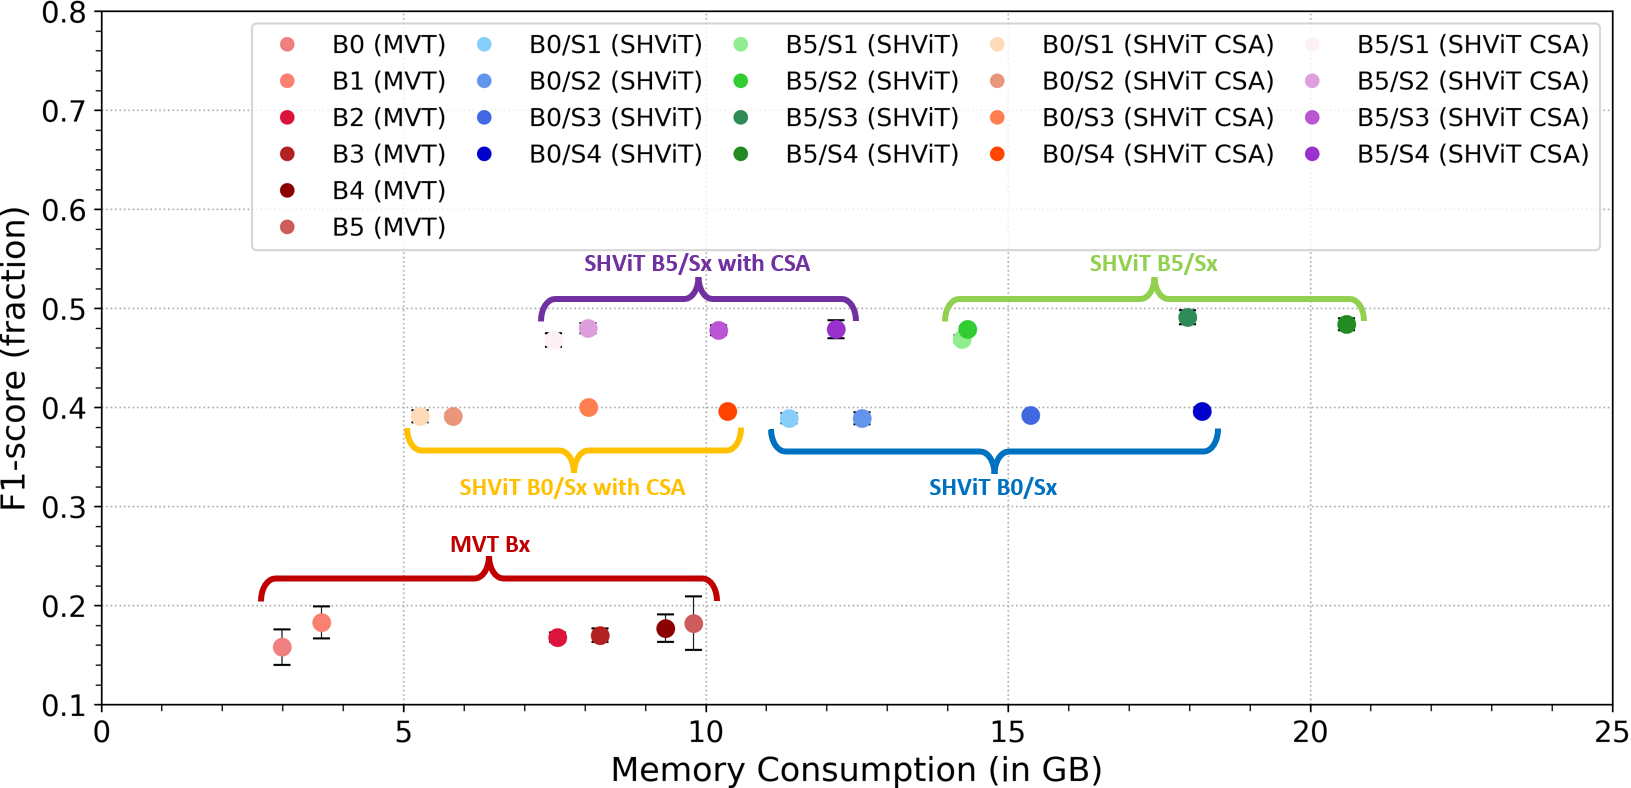
\includegraphics[width=1.0\textwidth]{./images/F1_vs_gpu_memory_w_text.png}
	\caption[F1-score versus GPU memory consumption]{F1-score versus GPU memory consumption for different parameter sets for MVT, SHViT, and SHViT with central self-attention (CSA)}
	\label{iou_vs_gpu_memory}
\end{figure}
The lowest group, with F1 values between 0.1 and  0.2, corresponds to models using the \gls{mvt} backbone, indicating limited segmentation performance on the \gls{3d} shoe scan task. The second group, with F1-score around 0.4, results from experiments using the \gls{shvit} backbone with the B0/Sx\footnote{see table \ref{tab:variants} on page \pageref{tab:variants}.} parameter settings, demonstrating improved accuracy compared to \gls{mvt} while maintaining relatively low memory usage. The highest accuracy group, with F1 values slightly below 0.5, is achieved using \gls{shvit} with the B5/Sx configuration, suggesting that deeper and more expressive backbone variants lead to significantly better segmentation performance, but this comes with increased memory consumption.

\medskip

While the standard \gls{shvit} models already outperform \gls{mvt} in terms of accuracy, they tend to consume more \acrshort{gpu} memory. However, introducing the central self-attention mechanism significantly reduces memory usage between 43\% and 54\% (for B0/Sx-configurations) and between 41\% and 47\% (for B5/Sx) without compromising segmentation performance. This highlights the central self-attention variant as a more efficient alternative, offering a favorable trade-off between computational cost and predictive accuracy.

\medskip

An intriguing observation from the experiment is the differing sensitivity of the two backbone types to their respective hyperparameter settings. For the standard SegFormer model with the \gls{mvt} backbone, the F1 accuracy improves noticeably when progressing from the B0 to the B5 configuration. This indicates that increasing model capacity through deeper and wider transformer layers positively impacts segmentation performance. In contrast, the \gls{shvit}-based models show relatively stable F1 performance across the different Sx configurations (S1 to S4), regardless of whether B0 or B5 decoding dimensions are used. This suggests that the \gls{shvit} backbone is less sensitive to internal architectural scaling and that even its smaller configurations are able to extract meaningful features from the \gls{3d} volumes effectively.

\medskip

It was initially expected that the \gls{mvt}-based SegFormer model would achieve significantly better results on the \gls{3d} shoe scan data, given its strong performance on \gls{2d} segmentation benchmarks. In \gls{2d} experiments, the \gls{mvt} backbone consistently produced high \gls{iou} values \cite{xie2021segformersimpleefficientdesign}. However, in this study, the \gls{mvt} model performed notably worse on the volumetric data, achieving only small \gls{iou} scores with 0.2 and below\footnote{For this comparison the \gls{iou} was also calculated.}. This performance gap suggests that while the \gls{mvt} architecture is well-suited for \gls{2d} spatial relationships, it does not generalize effectively to \gls{3d} volumetric data without further architectural adaptations.

\bigskip

Another noteworthy observation is the significant difference in the number of trainable parameters between the \gls{mvt}-based and \gls{shvit}-based models, as shown in figure \ref{iou_vs_train_parameters}. For the \gls{mvt} backbone, the number of parameters spans a wide range, from approximately 5 million in the B0 configuration up to around 120 million for B5. In contrast, all \gls{shvit}-based models, including those augmented with central self-attention, remain significantly more compact, with a maximum of approximately 20 million trainable parameters. This big decrease in model size shows the efficiency of the \gls{shvit} architecture, which achieves comparable or superior segmentation performance while maintaining a much lower parameter count, making it particularly attractive for resource-constrained environments.
\begin{figure}[H]
	\centering
	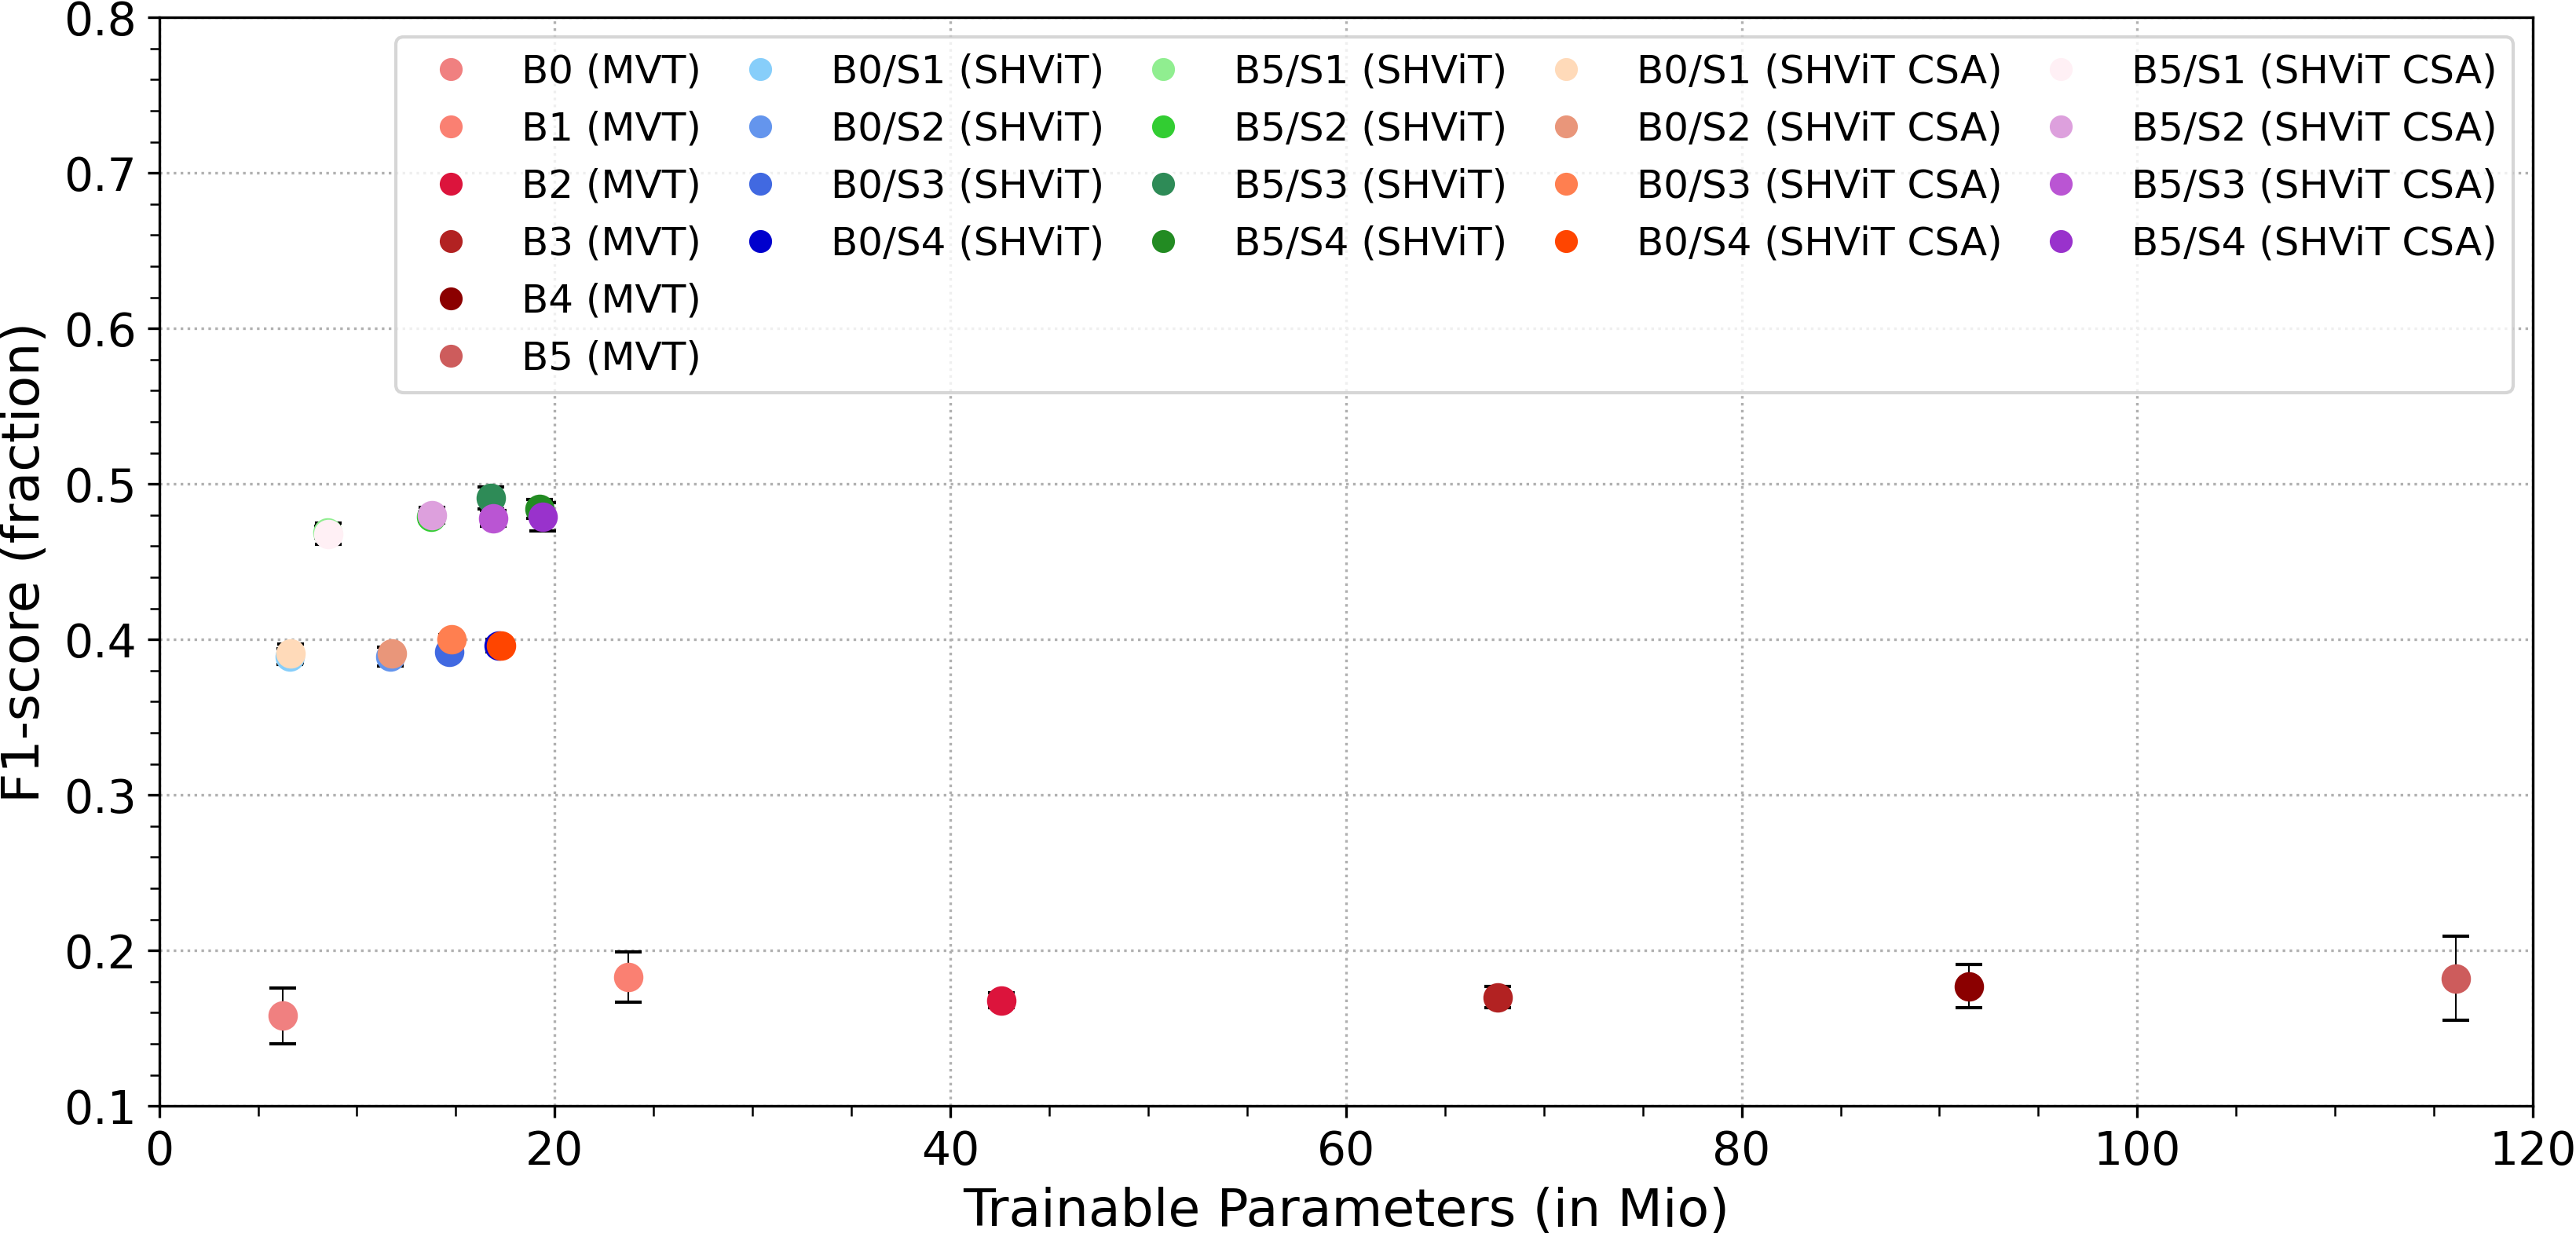
\includegraphics[width=1.0\textwidth]{./images/F1_vs_train_parameters.png}
	\caption[F1-score versus number of trainable parameters]{F1-score versus number of trainable parameters for different parameter sets for MVT, SHViT, and SHViT with central self-attention (CSA)}
	\label{iou_vs_train_parameters}
\end{figure}

Some results of the trained segmentation model on selected shoe volumes are shown in figure \ref{result_for_shvit_with_center_attention} for the \gls{shvit}-model with central self-attention and input volume size of {\tt (224,224,224)}. For each case, a central slice of the \gls{3d} volume is displayed, showing from left to right: the input image, the predicted segmentation, and the corresponding ground truth. These examples illustrate the model's performance in identifying and segmenting the relevant components within the shoe scans.

\medskip

For the subsequent experiments, the \gls{shvit} model with central self-attention and the B5/S2\footnote{see table \ref{tab:variants} on page \pageref{tab:variants}.} configuration was selected, as it provides a favorable balance between segmentation accuracy and memory efficiency in the initial comparison.

\begin{figure}[H]
	\centering
%	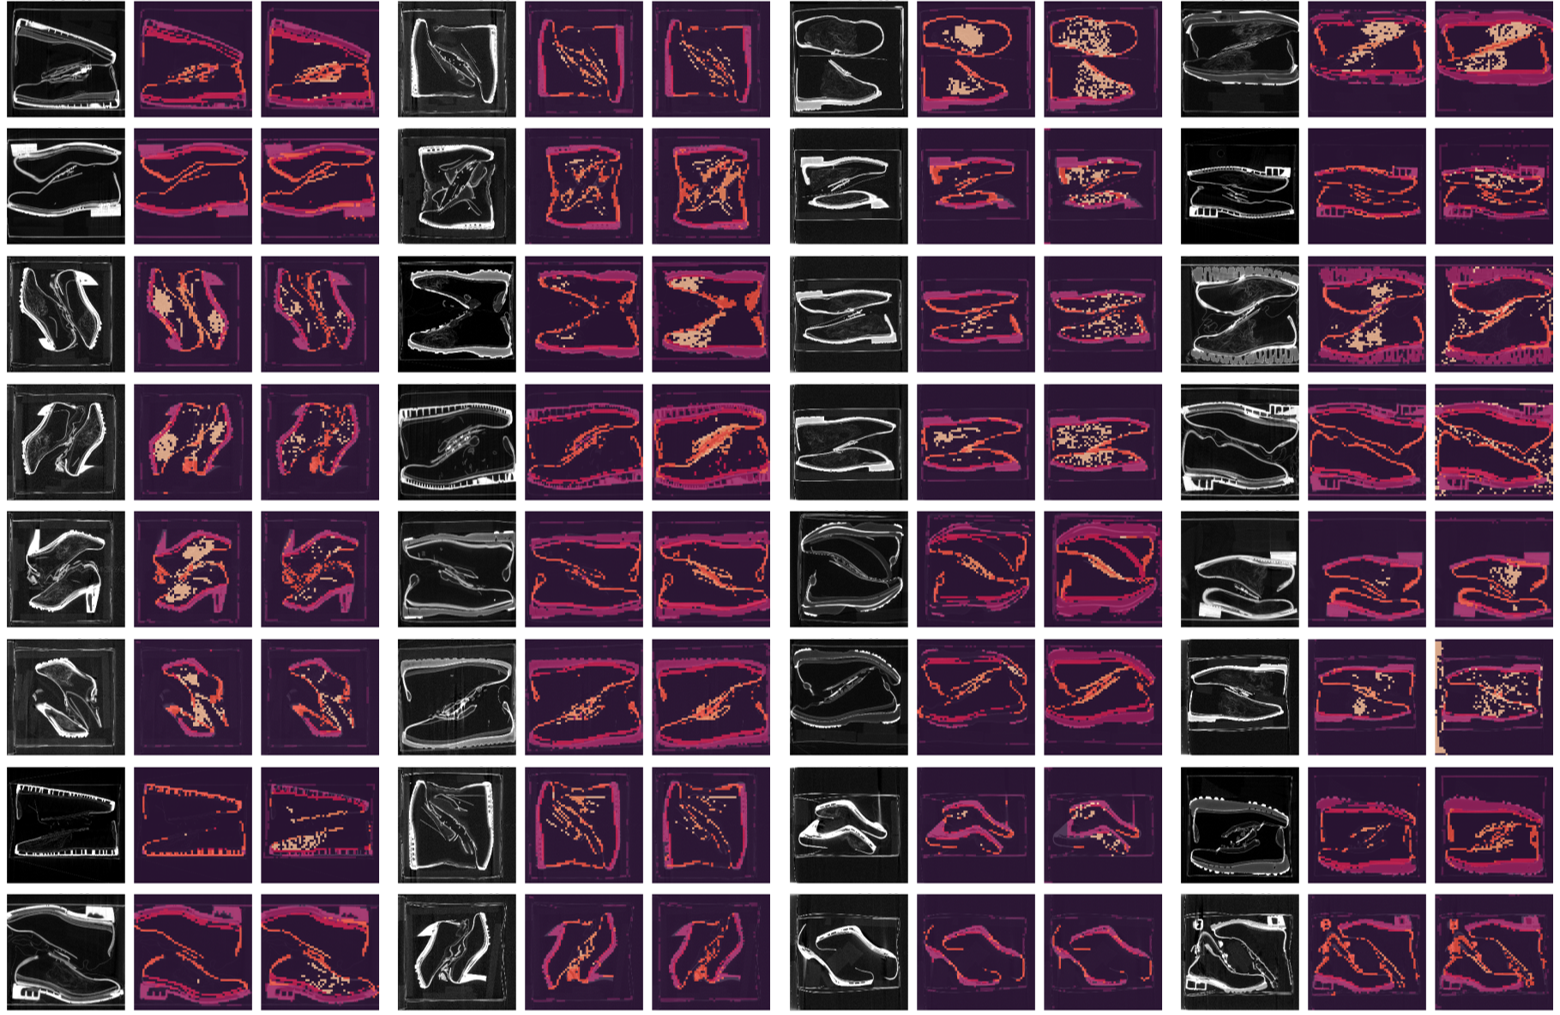
\includegraphics[width=1.0\textwidth]{./images/Shoes_224x224x224_B5S2.png}
%	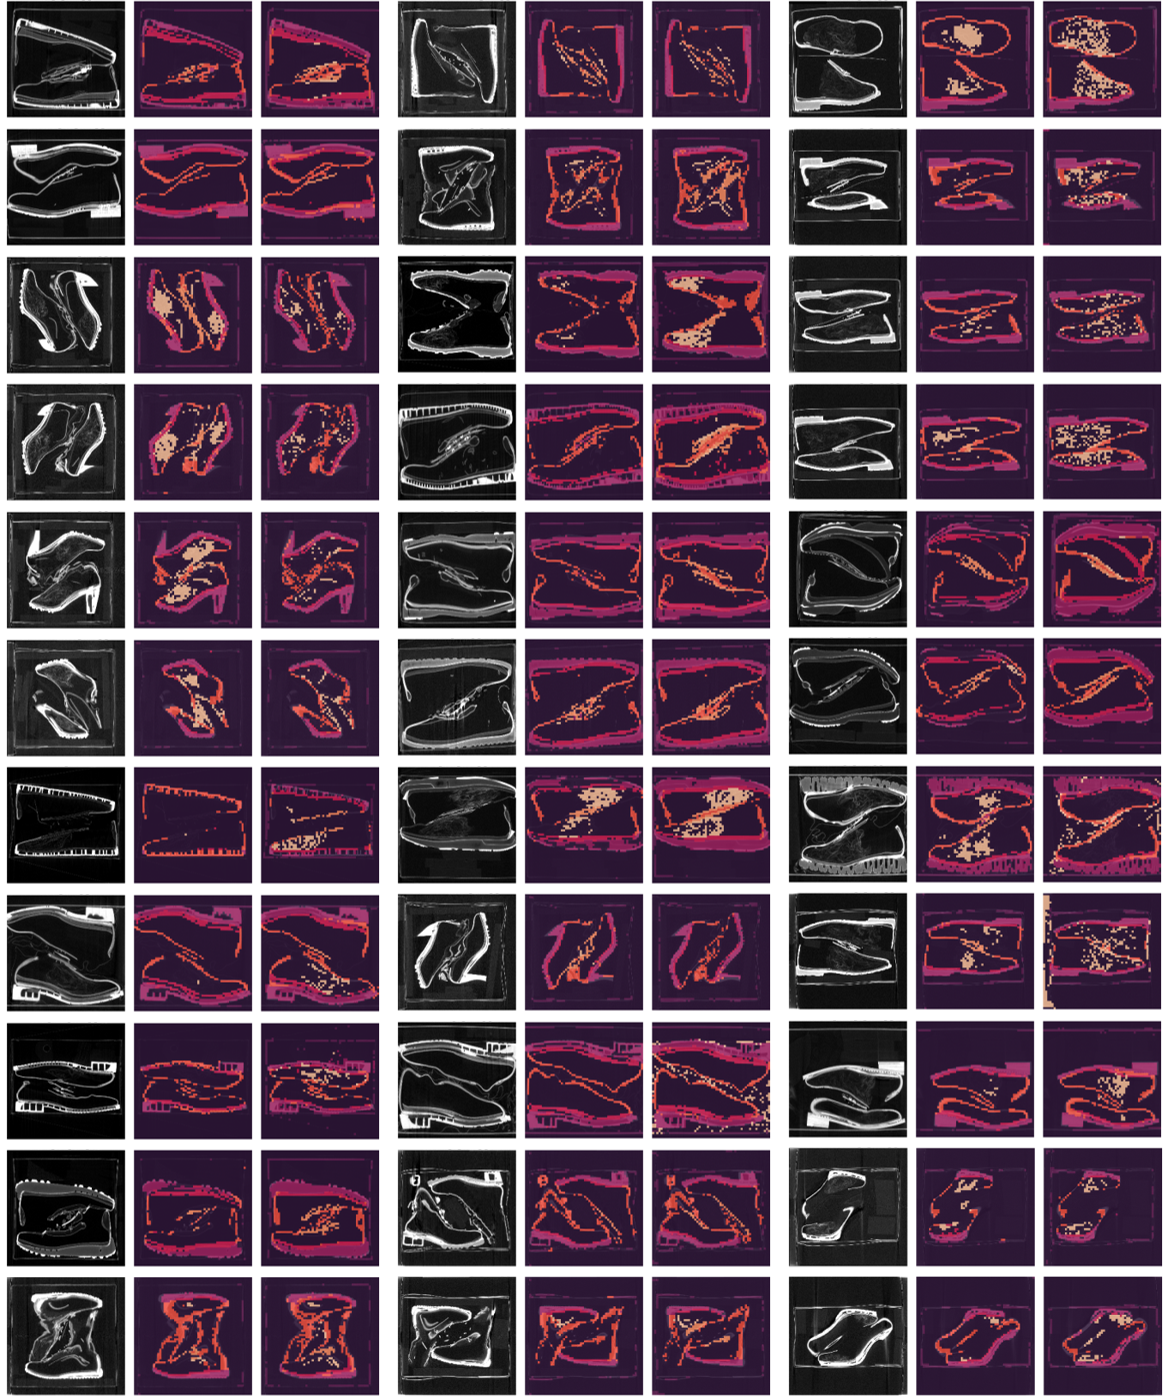
\includegraphics[width=1.0\textwidth]{./images/Shoes_224x224x224_B5S2_v2.png}
	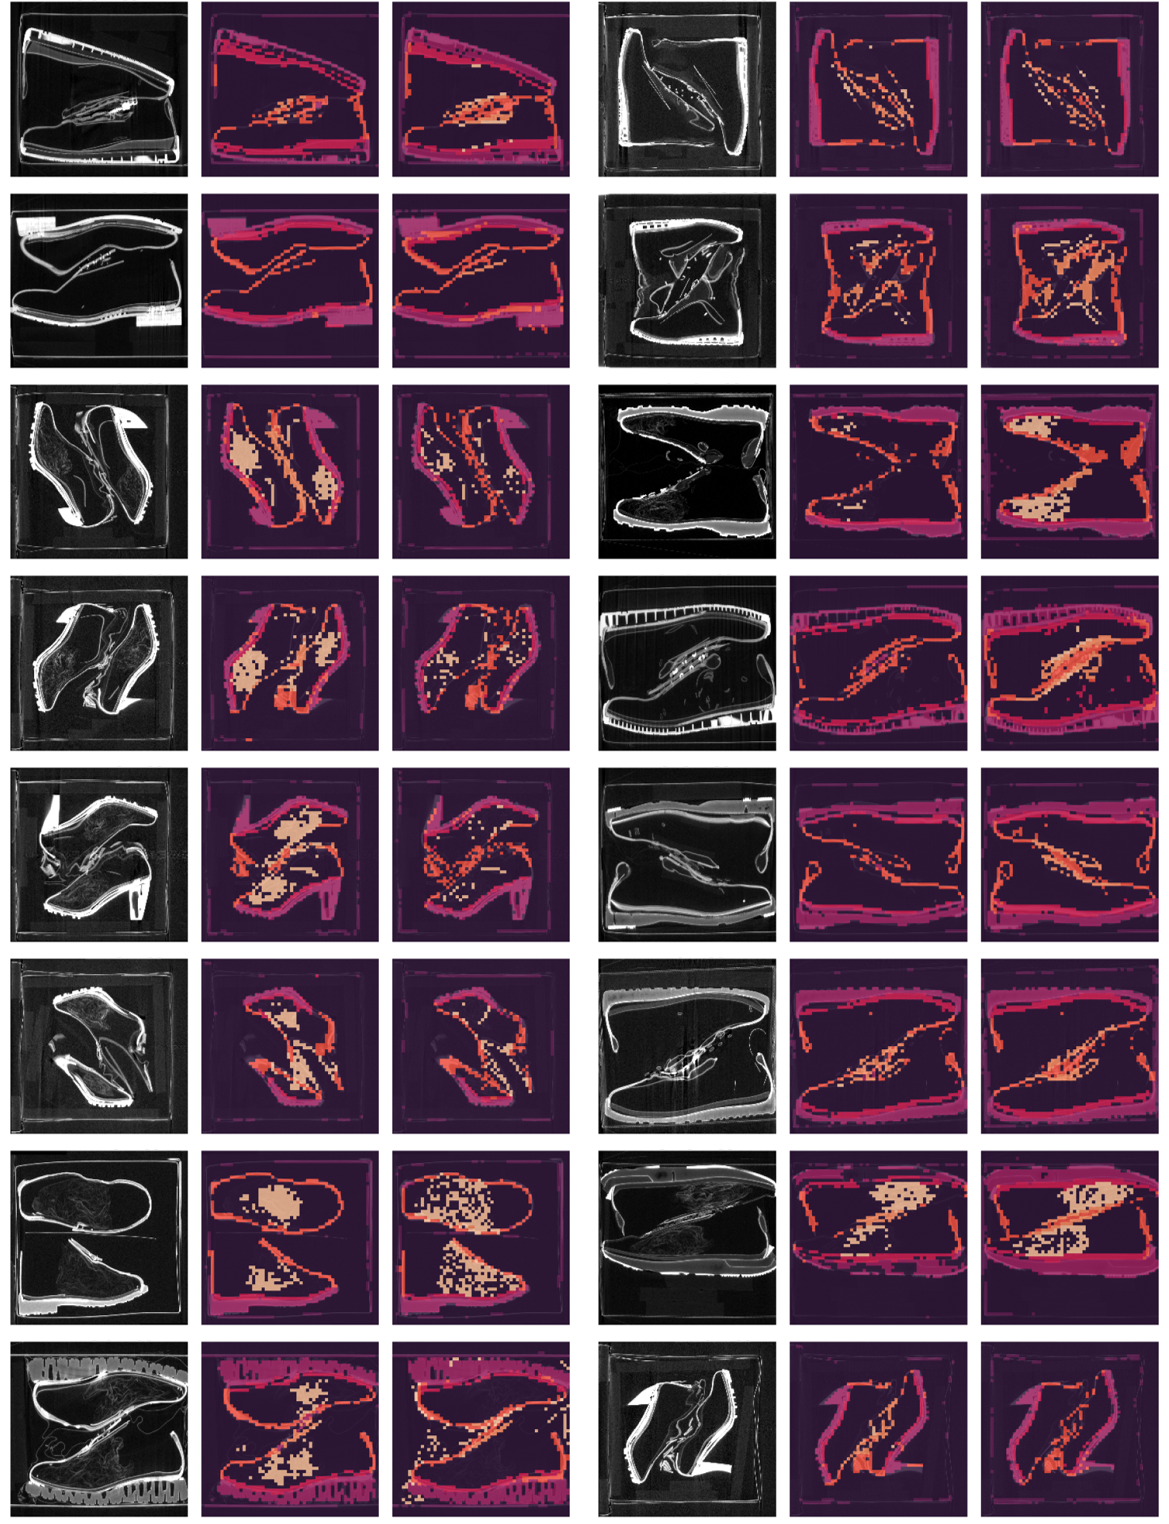
\includegraphics[width=1.0\textwidth]{./images/Shoes_224x224x224_B5S2_v3.png}
	
\includegraphics[width=0.9925\textwidth]{./images/color_legend_7_classes.png}
	\caption[Results of some shoes trained with the 3D-SHViT model with central self-attention]{Results of some shoes trained with the 3D-SHViT model with central self-attention. From left to right: the input image, the predicted segmentation, and the corresponding ground truth segmentation image for each of the two columns.}
	\label{result_for_shvit_with_center_attention}
\end{figure}



\section{Evaluation of Maximum Volume Size for SHViT on a 24\,GB GPU}
The second experiment aims to determine the maximum input volume size that can be processed by \gls{shvit}-based models under given hardware limitations. Understanding the scalability of the architecture is crucial for real-world applications, where high-resolution volumetric data is often desirable but constrained by \acrshort{gpu} memory capacity.

\medskip

By systematically increasing the input dimensions while monitoring memory usage, this analysis identifies the practical upper bounds for volume size on a 24\,GB \acrshort{gpu}. The results provide valuable insights into the efficiency of the \gls{shvit} architecture and its suitability for processing large-scale \gls{3d} inputs, especially in comparison to more memory-intensive transformer backbones.

\medskip

As demonstrated in the previous section, the \gls{shvit} model with central self-attention outperforms the other configurations in terms of segmentation accuracy and memory efficiency. Therefore, this model configuration is selected for the subsequent experiment to further explore its performance with different volume sizes.

\medskip

Figure \ref{iou_vs_vol_memory} shows the relationship between F1-score and \acrshort{gpu} memory consumption for different input volume sizes from the \gls{shvit} B5/S2-model. It can be observed that for very small volumes (e.g., {\tt (96,96,96)}, the F1-score is with 0.375 relatively low. As the volume size increases, the F1-score improves until it reaches a plateau at a volume size of {\tt (256,256,256)}. After this point, the F1-score remains flat, with only a very slight increase observed starting from a volume size of {\tt (320,320,320)}. The volume size of {\tt (352,352,352)} was not tested due to memory limitations, as it would have increased \gls{gpu}-memory usage to approximately 54\,GB.

\medskip

The lower F1-score at a volume size of {\tt (96,96,96)} may be attributed to both the lower resolution of the input volume and the relatively small size of the segment volume, which has a resolution of {\tt (24,24,24)}. This small segment volume limits the ability to capture fine details. As the input volume increases, the segment volume increases as well, leading to better performance. Table \ref{tab:volume_stages} illustrates the volume sizes at each stage of the \gls{shvit} model with 2 convolution layers in \gls{shvit} head, which already reduces the input size by a factor of 4.
\begin{figure}[H]
	\centering
	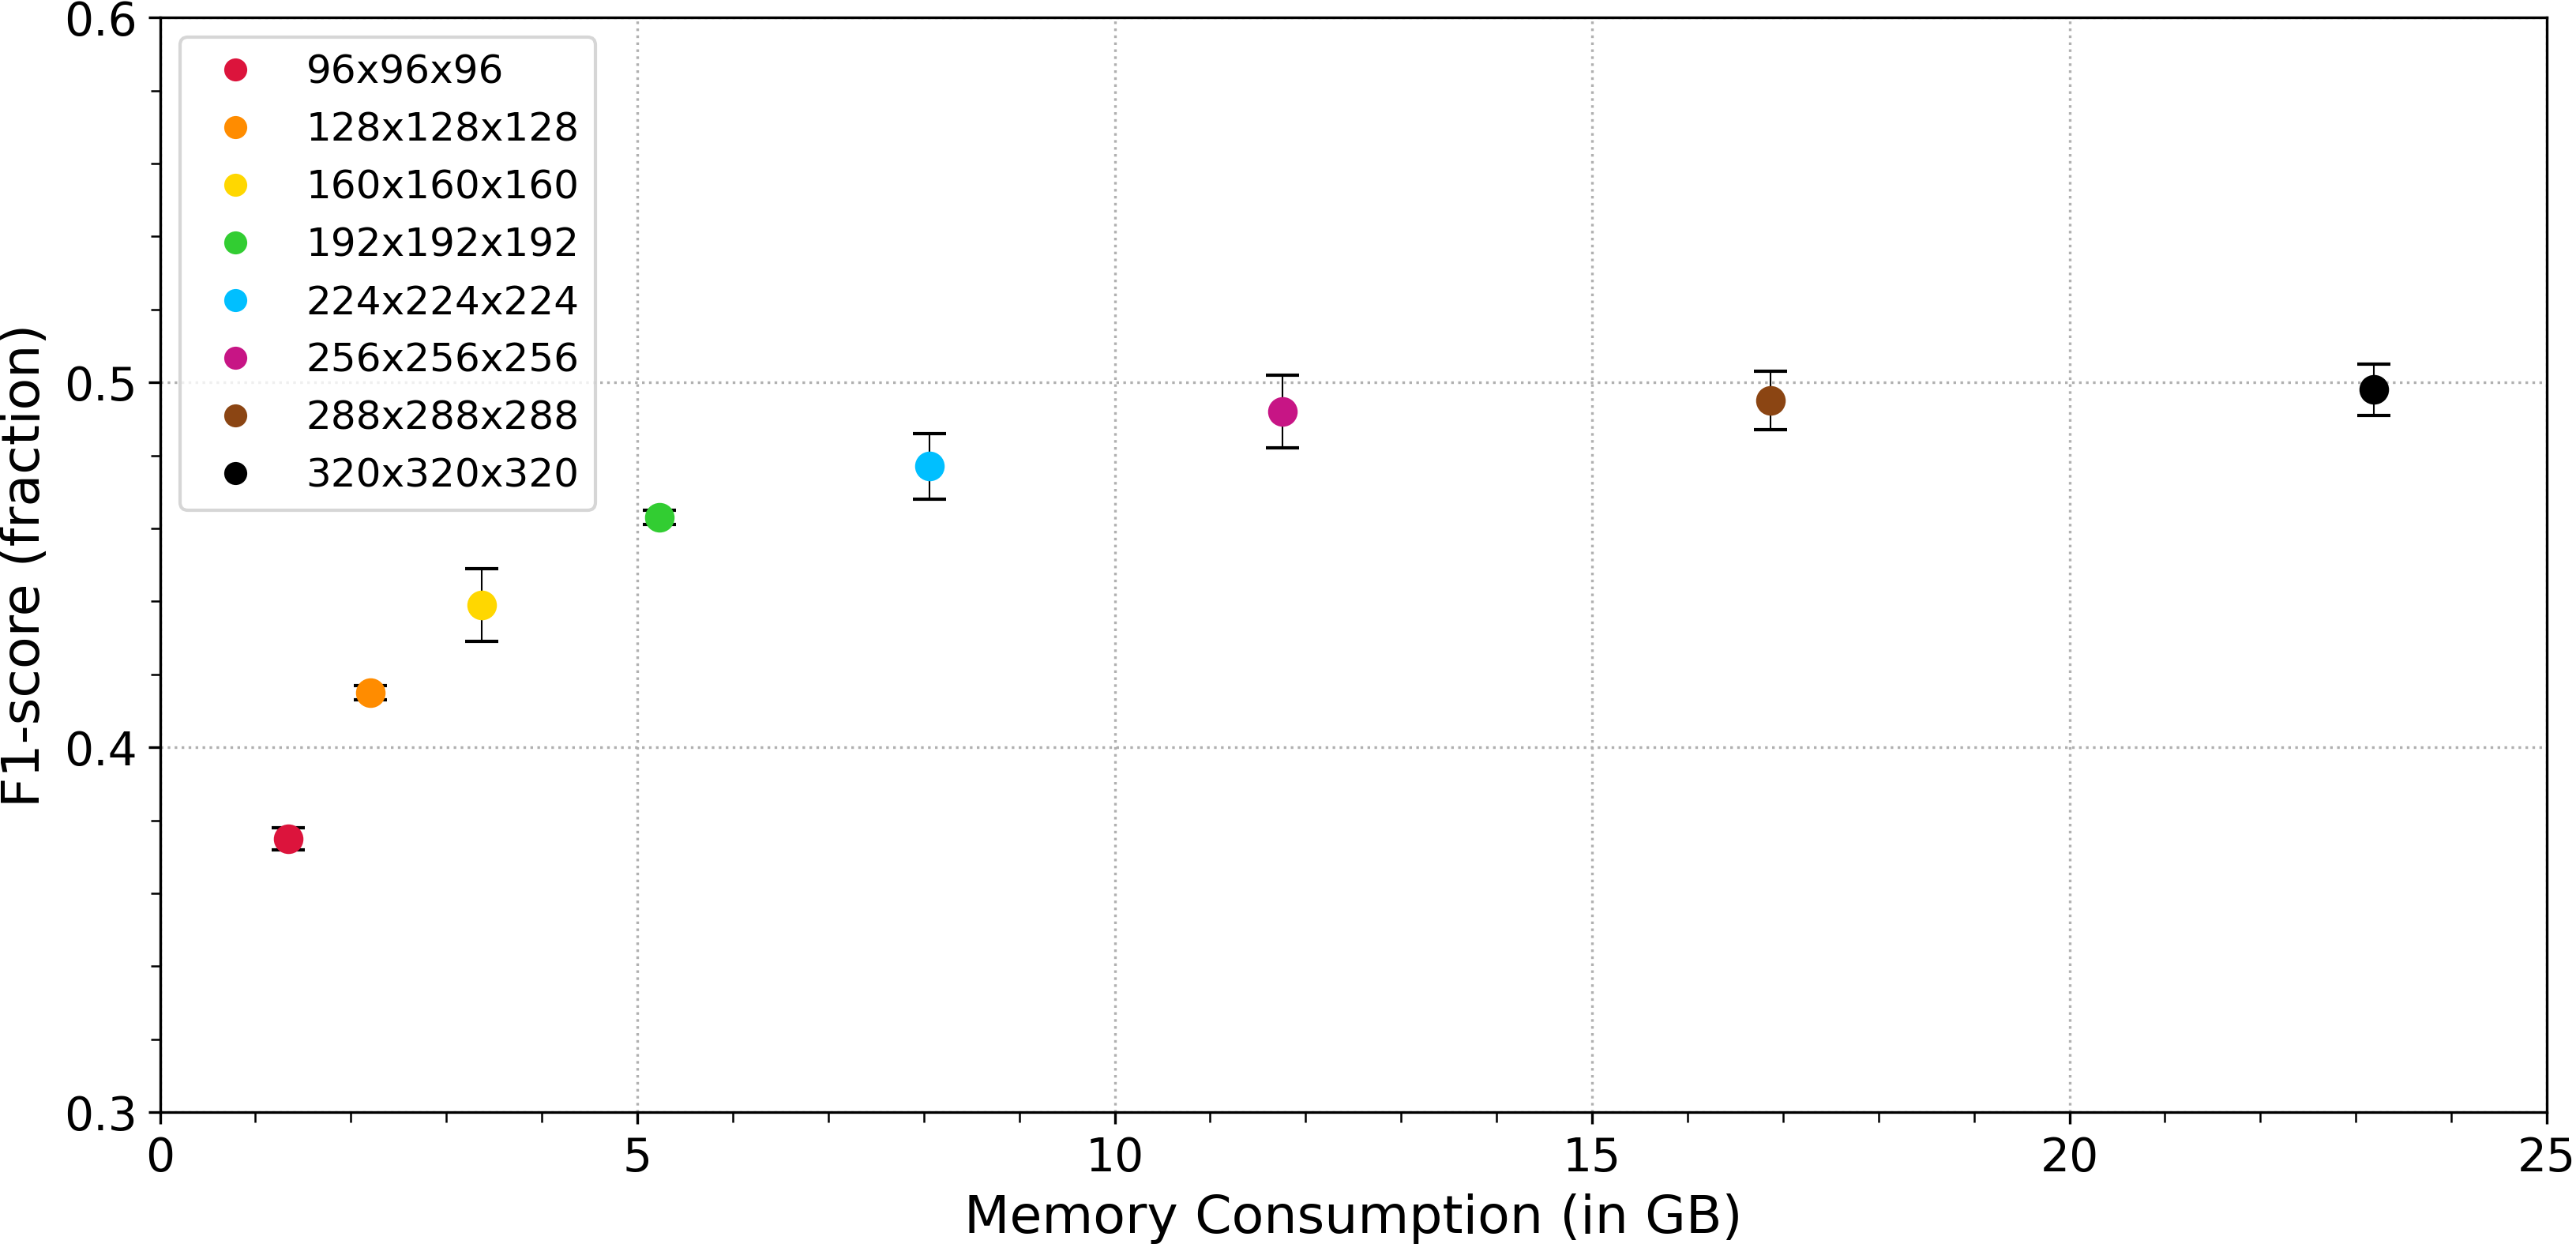
\includegraphics[width=1.0\textwidth]{./images/F1_vs_vol_memory.png}
	\caption[F1-score versus GPU memory consumption for different volume sizes]{F1-score versus GPU memory consumption for different volume sizes. The base model is SHViT B5/S2 with central self-attention.}
	\label{iou_vs_vol_memory}
\end{figure}

\begin{center}
\begin{threeparttable}[H]
	\begin{tabular}{c|cccc|c|c}
		\toprule
		\CellWithForcedBreak{volume \\ input \\ size} & \CellWithForcedBreak{size before \\ 1st stage} & \CellWithForcedBreak{size before \\ 2nd stage} & \CellWithForcedBreak{size before \\ 3rd stage} & \CellWithForcedBreak{size after \\ 3rd stage} & \CellWithForcedBreak{segment \\ volume \\ size} & \CellWithForcedBreak{max. \\ memory \\ consumption} \\
		\midrule
		\midrule
		96 & 24 & 24 & 12 &  6 & 24 & 1.34\,GB \\
		128 & 32 & 32 & 16 &  8 & 32 & 2.20\,GB \\
		160 & 40 & 40 & 20 &  10 & 40 & 3.37\,GB \\
		192 & 48 & 48 & 24 &  12 & 48 & 5.23\,GB \\
		{\bf 224} & {\bf 56} & {\bf 56} & {\bf 28} &  {\bf 14} & {\bf 56} & {\bf 8.05\,GB} \\
		256 & 64 & 64 & 32 &  16 & 64 & 11.76\,GB \\
		288 & 72 & 72 & 36 &  18 & 72 & 16.87\,GB \\
		320 & 80 & 80 & 40 & 20 & 80 & 23.19\,GB \\
		\midrule
		352 & 88 & 88 & 44 & 22 & 88 & >50\,GB \\
		\bottomrule
	\end{tabular}
	\caption[Overview of input volume sizes and their corresponding resolutions after each stage of the SHViT B5/S2-model]{Overview of input volume sizes and their corresponding resolutions after each stage of the SHViT B5/S2-model. The input volume is progressively reduced by convolutional layers (each with a stride of 2), and the resulting resolutions before/after each stage are shown. Between each stage is also a downsampling layer which reduces the volume by a factor of 2 (see figure \ref{Architecture_of_SHViT_Segformer} for details). The final segmentation volume is constructed from the outputs in the SegFormer decoder of the three stages of SHViT.}
	\label{tab:volume_stages}	
\end{threeparttable}
\end{center}

It is important to note that the segment output is derived from the last three stages of the \gls{shvit} model, meaning the input volume size of the first stage dictates the size of the segment output. Furthermore, not all volume sizes are feasible due to the structure of the model. After each stage, a convolution layer reduces the volume size by a factor of 2. Therefore, the output size at each stage should always be even (except for the last stage where it could also be uneven), as the upsampling in the \gls{mlp} layer and subsequent concatenation with previous layers require matching dimensions.

\medskip

Figure \ref{comparison_segmentations_for_different_volume_sizes} shows the predicted segmentation images for three different input volume sizes.

\begin{figure}[H]
	\centering
	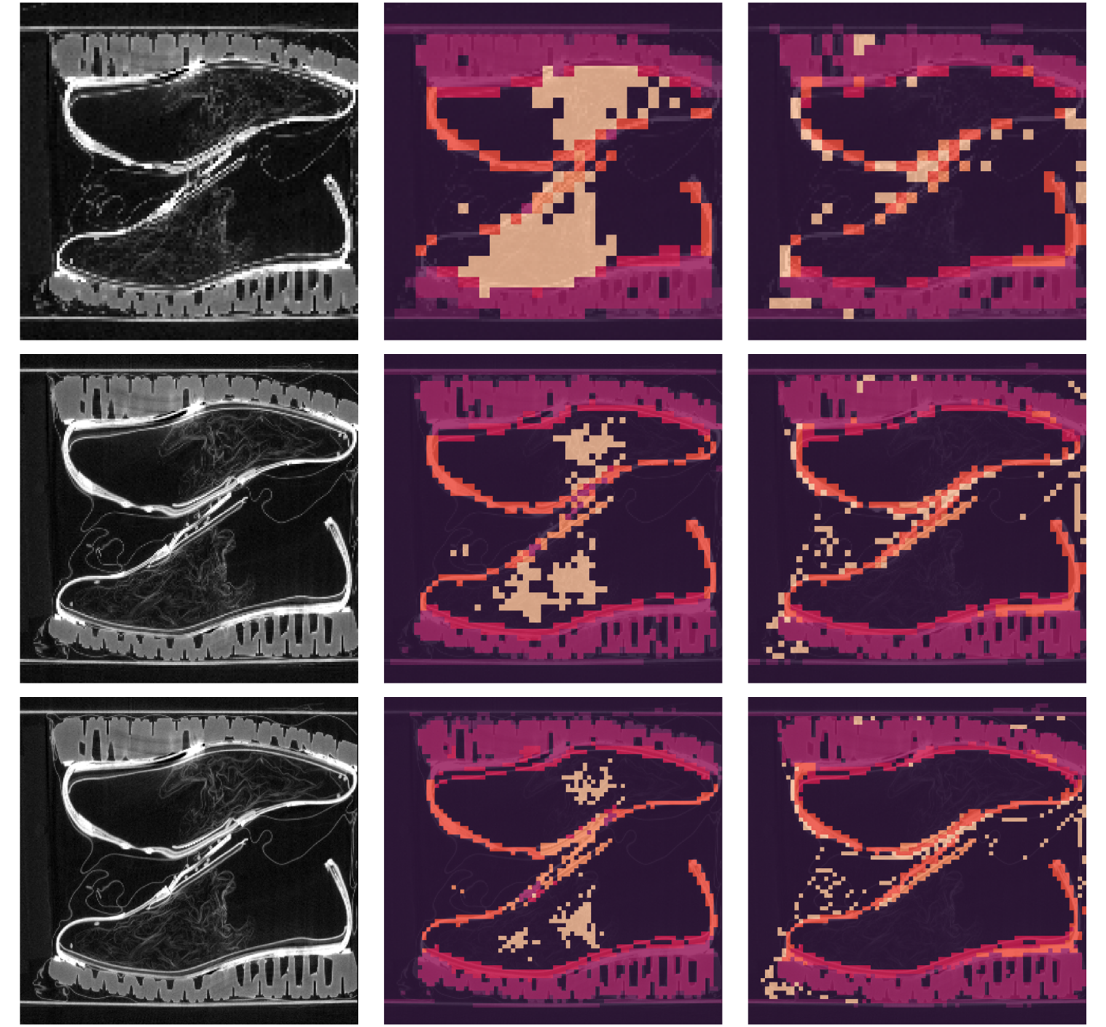
\includegraphics[width=0.7\textwidth]{./images/Shoepassion_40_down2_2_2_128-224-320.png}
	
\includegraphics[width=0.8\textwidth]{./images/color_legend_7_classes_v2.png}
	\caption[Comparison of the results with different volume sizes]{Comparison of the results with different volume sizes for {\tt Shoepassion\_40\_down2\_2\_2}. From left to right: the input image, the predicted segmentation, and the corresponding ground truth segmentation image. From top to bottom: input sizes increase from {\tt (128,128,128)} to {\tt (224,224,224)} and {\tt (320,320,320)}, with corresponding segmentation sizes from {\tt (32,32,32)} to {\tt (56,56,56)} and {\tt (80,80,80)}. For this pair of shoes, the predicted segmentation includes the filling material (visible inside the shoe), which is absent in the ground truth image, pointing to a potential inconsistency or omission in the labeling of this particular instance.}
	\label{comparison_segmentations_for_different_volume_sizes}
\end{figure}

The visualizations demonstrate how the resolution of the segmentation output varies with the input size. In particular, the coarseness of the segmentation at lower resolutions becomes evident, highlighting the limitations of small input volumes in accurately capturing fine structural details.


\section{Impact of Convolutional Depth on F1-score}
In this section, the influence of the number of convolutional layers $N$ in the \gls{shvit} segmentation head (overlay patch embedding, see figure \ref{Architecture_of_SHViT}) on both segmentation accuracy and \acrshort{gpu} memory consumption is analyzed. The convolutional layers in the head are responsible for processing the output features from the backbone and generating the final segmentation volume. By adjusting the depth of these layers, the trade-off between model complexity, segmentation quality (measured by F1-score), and computational efficiency is explored. 

\medskip

Each convolutional layer in the \gls{shvit} head reduces the spatial dimensions of the input by a factor of 2 due to the use of a stride of 2. Consequently, the output shape after $N$ convolutional layers can be calculated using the following formula:
\begin{equation}
\text{Output Shape} = \left(\frac{D}{2^N},\frac{H}{2^N},\frac{W}{2^N}\right)
\end{equation}
where $D$, $H$, and $W$ represent the depth, height, and width of the input volume, respectively, and $N$ is the number of convolutional layers. This relationship is essential for selecting compatible input sizes and ensuring consistent output dimensions across experiments.

\medskip

For this experiment, only those configurations of the \gls{shvit} head were evaluated that were feasible within available 24\,GB \acrshort{gpu} memory limits. Specifically, three variants with 1, 2, and 3 convolutional layers were tested\footnote{In addition to the high \acrshort{gpu} memory consumption associated with using 4 convolutional layers and a large input volume, the resulting file size per shoe amounts to approximately 2.7\,GB. This significantly increases the computational burden, not only in terms of memory usage but also in terms of training time, as the large volume files must be read from the \acrshort{ssd} for each epoch. This I/O overhead further limits the practicality of such configurations in resource-constrained environments.}. To ensure fair comparison across all configurations, the input volume size was adjusted so that the resulting segmentation output size remained constant at {\tt (56,56,56)}. This design choice eliminates potential confounding effects caused by differing output resolutions and enables a focused analysis of how convolutional depth influences segmentation performance and memory usage. Table~\ref{tab:volume_layers} summarizes the evaluated setups.

\begin{center}
	\begin{threeparttable}[H]
		\begin{tabular}{c|c|c|c|c}
			\toprule
			\CellWithForcedBreak{number of \\ conv layers N} & \CellWithForcedBreak{volume \\ input size} & \CellWithForcedBreak{size after \\ N conv layers} & \CellWithForcedBreak{segment \\ volume size} & \CellWithForcedBreak{max. memory \\ consumption} \\
			\midrule
			\midrule
			1 & 112 & 56 & 56 & 7.62\,GB \\
			{\bf 2} & {\bf 224} & {\bf 56} & {\bf 56} & {\bf 8.05\,GB} \\
			3 & 448 & 56 & 56 & 13.07\,GB \\
			\midrule
			4 & 896 & 56 & 56 & >50\,GB \\
			\bottomrule
		\end{tabular}
		\caption[Overview of input volume sizes and their corresponding segmentation resolutions of the SHViT B5/S2-model for different numbers of conv.~layers]{Overview of input volume sizes and their corresponding segmentation resolutions of the SHViT B5/S2-model for different numbers of convolutional layers.}
		\label{tab:volume_layers}
	\end{threeparttable}
\end{center}

The following figure \ref{iou_vs_layers_memory} illustrates the relationship between F1-score and \acrshort{gpu} memory consumption for three different \gls{shvit} head configurations. The configuration with only one convolutional layer gives the lowest accuracy, likely due to the reduced input resolution. 
\begin{figure}[H]
	\centering
	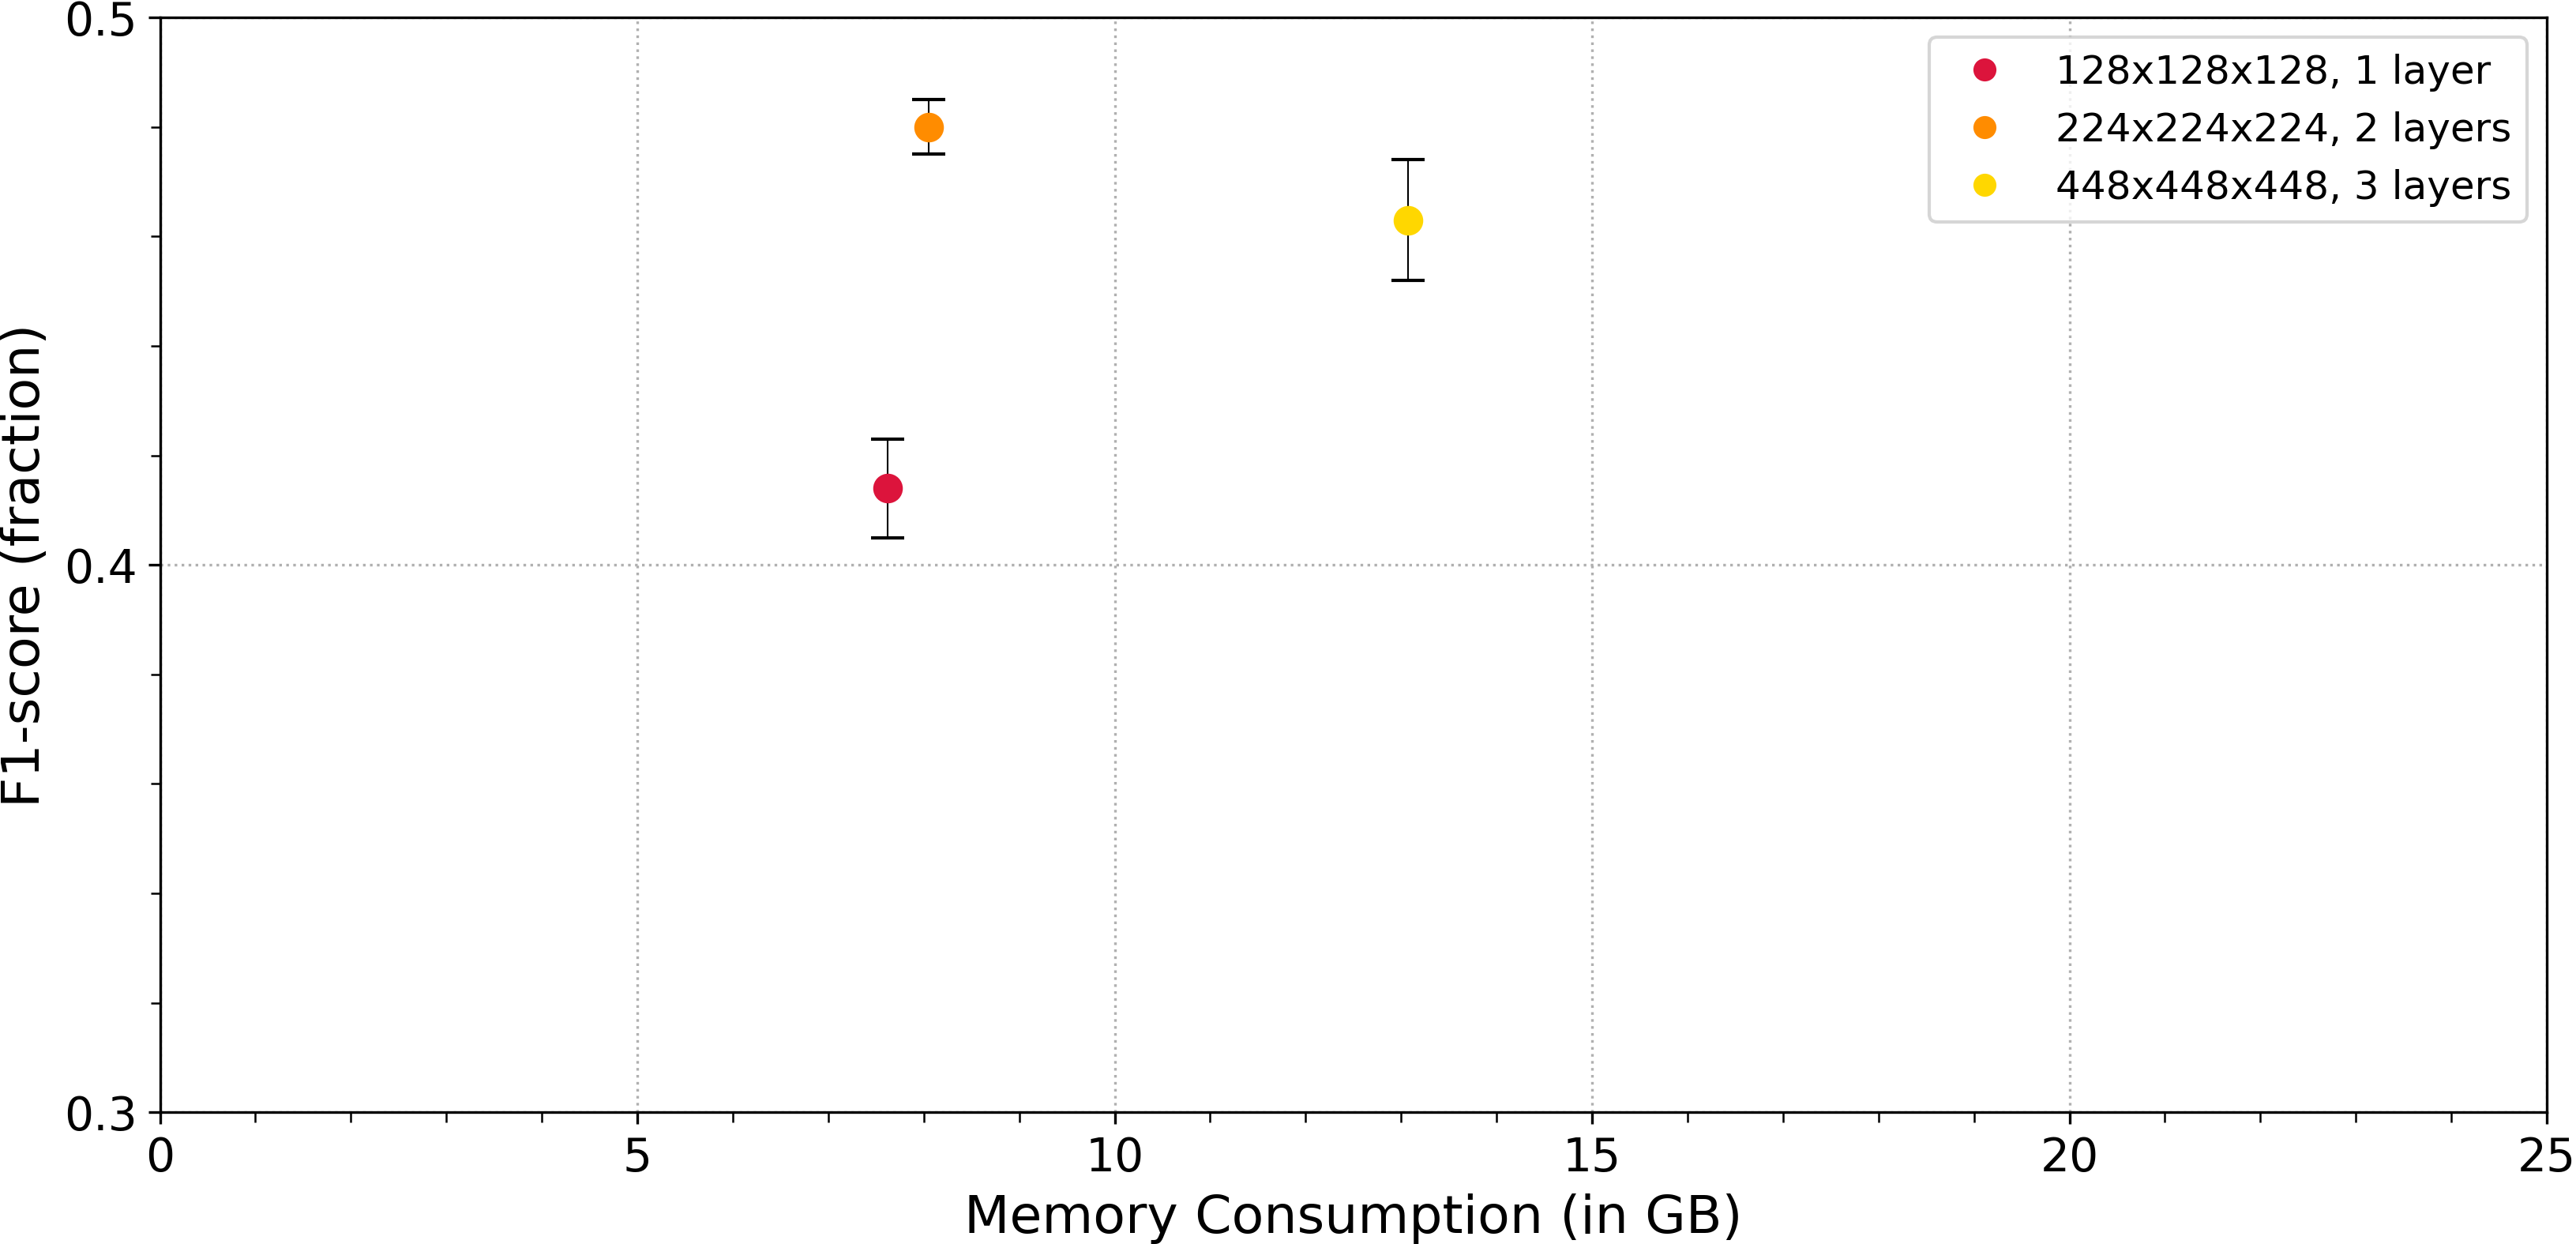
\includegraphics[width=1.0\textwidth]{./images/F1_vs_layers_memory.png}
	\caption[F1-score versus GPU memory consumption for different numbers of conv.~layers]{F1-score versus GPU memory consumption for different numbers of convolutional layers and volume sizes, keeping segmentation volume the same. The experiment with 4 convolutional layers was not executed due to very high memory demand.}
	\label{iou_vs_layers_memory}
\end{figure}
Interestingly, the configuration with two convolutional layers outperforms the one with three layers, which was not anticipated. The three-layer configuration's results, however, show a notably larger error bar compared to the others, indicating higher variance between runs. This suggests that the observed trend may not be reliable. Additional training runs could help to reduce the variance and provide more conclusive evidence regarding the optimal number of convolutional layers.



\section{Effects of Kernel Size on F1-score and Memory}
This experiment was conducted to examine the impact of the kernel size used in the central self-attention block on segmentation performance. The kernel size determines the spatial extent over which attention is applied and thus influences the model's ability to capture contextual information. Kernel sizes of 1, 3, 5, and 7 were evaluated for the standard  \gls{shvit}-SegFormer B5/S2-model with central self-attention and 2 convolution layers and an input size of {\tt (224,224,224)}, and the corresponding results illustrating the relationship between F1-score and \acrshort{gpu} memory usage are shown in figure \ref{iou_vs_kernel_memory}. 
\begin{figure}[H]
	\centering
	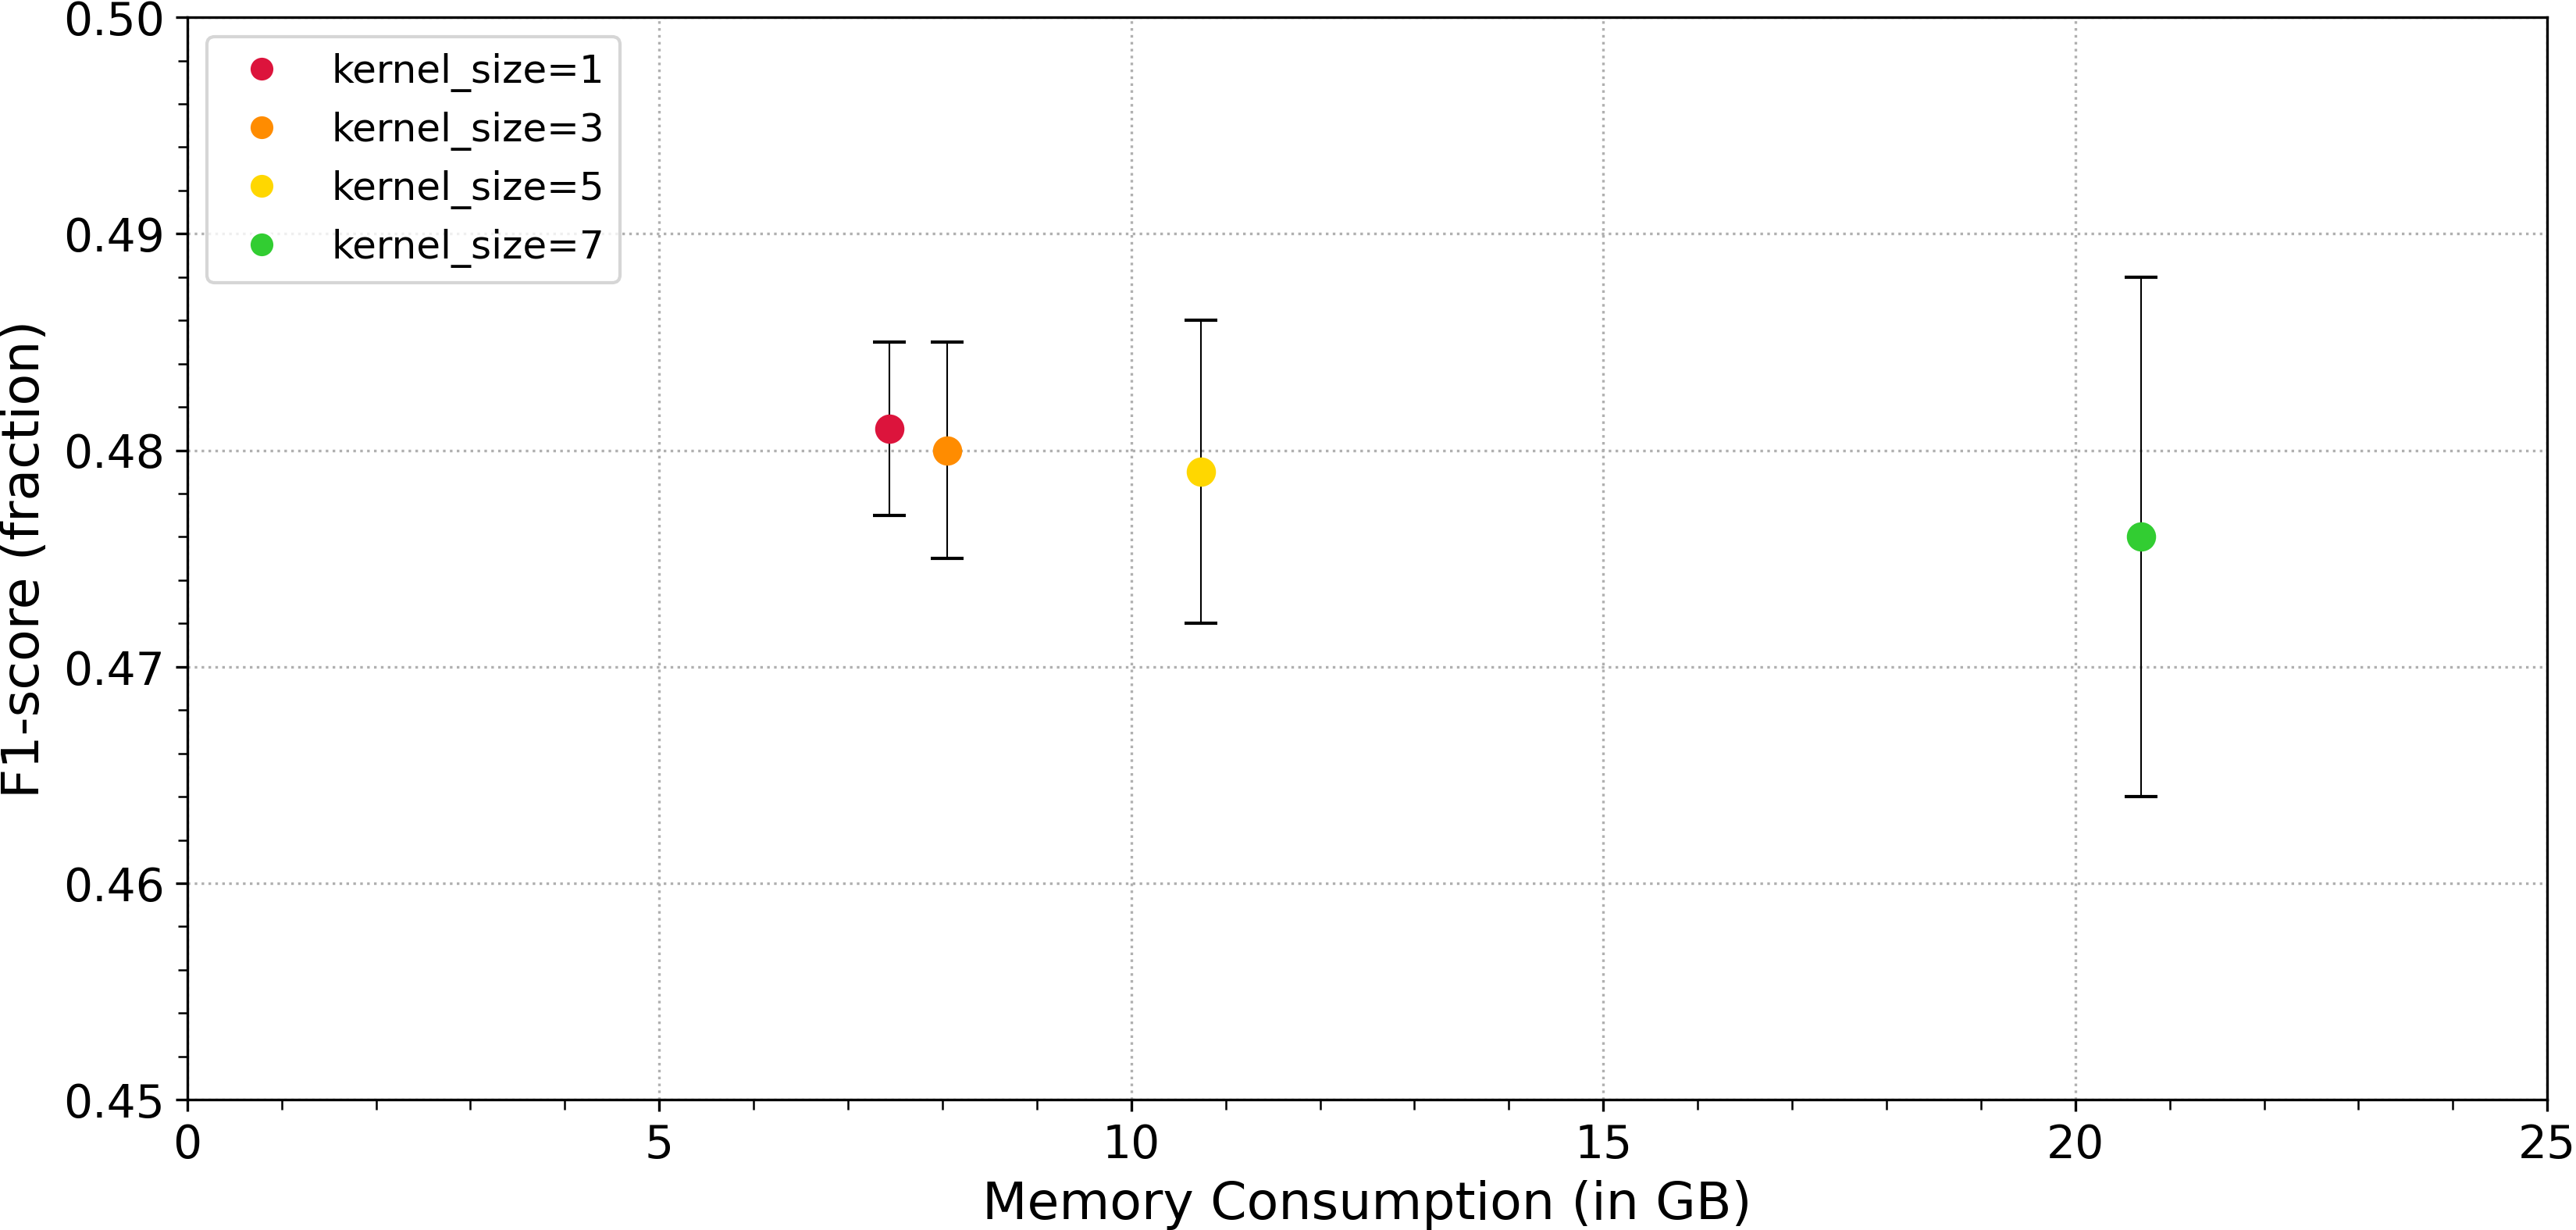
\includegraphics[width=1.0\textwidth]{./images/F1_vs_kernel_memory.png}
	\caption[F1-score versus GPU memory consumption for different kernel sizes]{F1-score versus GPU memory consumption for different kernel sizes.}
	\label{iou_vs_kernel_memory}
\end{figure}
A clear trend can be observed: the F1-score gradually decreases from {\tt kernel\_size=1} to {\tt kernel\_size=7}, with the error bar for {\tt kernel\_size=7} being noticeably larger than for other sizes. However, since the error bars overlap, it is difficult to confidently determine a statistically significant winner based solely on performance metrics. While {\tt kernel\_size=1} achieved the highest F1-score, followed closely by {\tt kernel\_size=3}, the marginal improvement with $1 \times 1$ kernels does not justify the loss of spatial modeling capability inherent in $3 \times 3$ kernels. Literature suggests that spatial context awareness enhances generalization performance, especially to unseen data, through the learning of spatially-coherent features rather than point-wise transformations \cite{he2015deepresiduallearningimage, simonyan2015deepconvolutionalnetworkslargescale, chollet2017xception}. In addition, training time per epoch increases substantially with larger kernels, rising from approximately 13 seconds for {\tt kernel\_size=1} to 51 seconds for {\tt kernel\_size=5}, and reaching 415 seconds for {\tt kernel\_size=7}. Considering both performance trends and the importance of spatial modeling capability, this study adopts {\tt kernel\_size=3} as the optimal configuration and recommends this setting for future experiments.

\medskip

In conclusion, these results showed that smaller attention kernel sizes led to higher F1-score than larger ones, a result which was not expected at first. However, literature suggests that smaller local attention windows are better at capturing fine structural details, which is especially important in \gls{3d} (medical) segmentation tasks. Studies such as \cite{Huang_2024, wu2024fewshotmedicalimagesegmentation, app142311365} support this hypothesis by showing that small-window attention helps preserve local texture and boundary precision, often leading to improved segmentation accuracy. These findings, well-established for convolutional kernels, suggest that attention mechanisms may benefit similarly from smaller kernel sizes, providing a theoretical foundation for the observed experimental results.

\medskip

As explained in section \ref{Transformer_Attention_Mechanisms}, the \gls{shcsa} block processes volumes of size {\tt (28,28,28)}, which are already relatively small. In this context, larger kernel sizes are less effective at capturing fine details.




\section[3D SHViT Segformer versus Residual SE UNet]{Segmentation performance: 3D SHViT Segformer versus Residual Squeeze and Excitation (SE) UNet}
To evaluate the segmentation performance and validate the \gls{3d} \gls{shvit} Segformer model, four distinct experiments were carried out. These experiments enabled a side-by-side comparison between the Residual Squeeze and Excitation (SE) UNet \cite{contribution_martin_leipert} and the \gls{shvit} Segformer architecture across different segmentation tasks. Performance evaluation is based on the F1-score calculated for individual semantic segments.

\medskip

This comparative analysis will provide insights into the relative strengths and limitations of convolutional versus transformer-based approaches for semantic segmentation tasks. To ensure a fair and direct comparison, both models use identical input specifications with volumetric data of {\tt (256,256,256)} voxels. The \gls{shvit} model is configured with hyperparameter settings of B5/S2 with central self-attention, and {\tt kernel\_size=3}, representing a balanced configuration between model complexity and computational efficiency. 


\subsection{Experiments 1-3: Comparative Analysis with Published Work}
The first three experiments were designed to replicate and compare \gls{3d} \gls{shvit} results with those reported in the existing literature \cite{contribution_martin_leipert}. These experiments serve as a benchmark to validate the implementation and ensure reproducibility of previously published findings. Each experiment follows the same methodology as the reference paper, enabling a direct performance comparison under identical conditions. The following tables summarize the obtained results.

\begin{center}
	\begin{threeparttable}[H]
		\begin{tabular}{lcc}
			\toprule[1.5pt]  
			& \multicolumn{2}{c}{Network} \\
			\multicolumn{1}{l}{F1-score} & {Residual SE UNet} & {SHViT Segformer} \\
			\midrule
			\midrule
			Total              & $0.821$ & $0.717 \pm 0.009$ \\
			\midrule
			Background         & $0.991$ & $0.958 \pm 0.002$ \\
			Shoe               & $0.882$ & $0.748 \pm 0.009$ \\
			Packaging Material & $0.589$ & $0.445 \pm 0.007$ \\
			\bottomrule
		\end{tabular}
		\captionsetup{width=0.95\textwidth}
		%		\captionsetup{width=\textwidth}
		\caption[Comparison of segmentation performance (F1-scores) between the Residual SE UNet and SHViT Segformer models across three different classes]{Experiment 1: Comparison of segmentation performance (F1-scores) between the Residual SE UNet and SHViT Segformer models across three different classes. The UNet model consistently outperforms SHViT Segformer, particularly for the \enquote{Shoe} and \enquote{Packaging Material} categories. Data for Residual SE UNet are taken from Table 2 \cite{contribution_martin_leipert}.}
		\label{tab:paper_3_segments}
	\end{threeparttable}
\end{center}

The results indicate that in all three comparative cases, the \gls{shvit} model demonstrates suboptimal performance in segmenting the defined segmentation classes, revealing challenges in the transformer-based approach for this specific application domain. Since the total F1-score is the averaged score of all segmentation classes, a poor result in one (or more) classes has a significant impact on the final score. 

\medskip 

Figure \ref{Paper_3Segments} shows the prediction results from the experiment using three segmentation classes, with images achieving high F1-scores displayed on the left and those with low F1-scores on the right.

\begin{figure}[H]
	\centering
	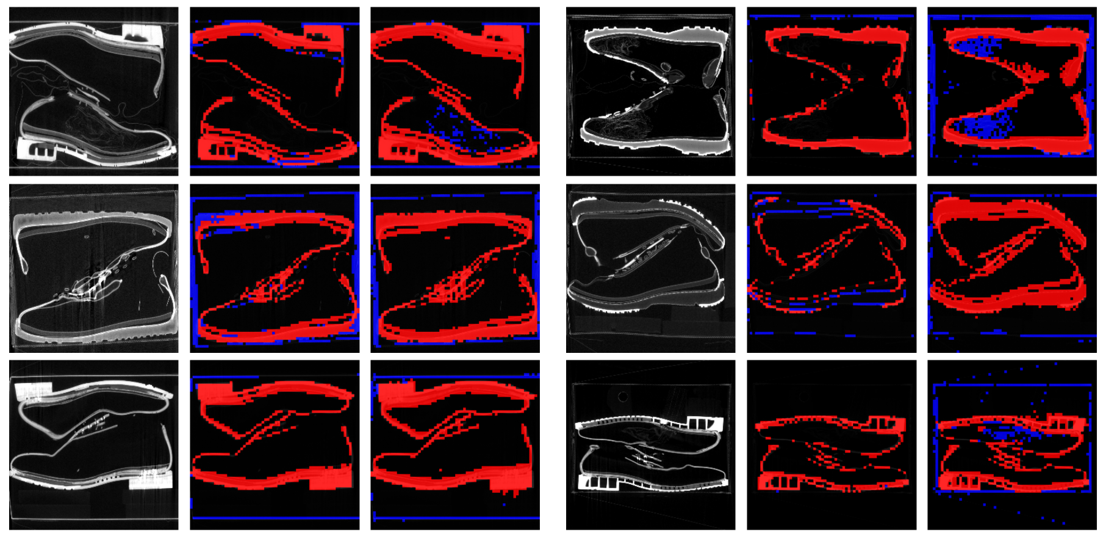
\includegraphics[width=1.0\textwidth]{./images/Paper_3Segments.png}
	
\includegraphics[width=0.9\textwidth]{./images/color_legend_3_classes.png}
	\caption[Results of shoes with 3 segments: background, shoe, and packaging material]{Results of shoes with 3 segments: background, shoe, and packaging material. From left to right: the input image, the predicted segmentation, and the corresponding ground truth segmentation image for each of the two columns. The images on the left have high overal F1-score ({\tt \small Bruschi\_down2\_2\_2: 0.829 [0.971, 0.840, 0.677]\footnotemark; Camper\_down2\_2\_2: 0.833 [0.948, 0.811, 0.740]; Herrenschuh\_43p5\_down2\_2\_2: 0.834 [0.968, 0.852, 0.682]}), the images on the right have a low F1-score ({\tt \small McKinley\_Anton\_down2\_2\_2: 0.620 [0.963, 0.750, 0.147]; Puma\_Silver\_down2\_2\_2: 0.659 [0.923, 0.487, 0.566]; Schuh\_Martin\_down2\_2\_2: 0.602 [0.977, 0.807, 0.023]}).}
	\label{Paper_3Segments}
\end{figure}
\footnotetext{{The order of these numbers are: total F1-score of the volume, in brackets the F1-score of background, shoe, and packaging material.}}

The background is detected with high confidence, typically achieving F1-scores well above 0.9 due to its large volume. The shoe is generally segmented well, while cardboard and packaging material show a higher standard deviation of nearly 0.2\footnote{The value of 0.2 should not be confused with the 0.007 in Table \ref{tab:paper_3_segments}. The latter is the standard deviation of mean values across five runs, while 0.2 reflects the deviation of packaging material across all volumes in the shoe dataset.}, likely because these relatively small regions are more difficult for the \gls{shvit} model to detect accurately.

\medskip

Experiments 2 and 3 use the same model architectures but modify the segmentation class definitions: experiment 2 simplifies the task to binary segmentation, while experiment 3 introduces four distinct classes.

\begin{center}
	\begin{threeparttable}[H]
		\begin{tabular}{lcc}
			\toprule[1.5pt]  
			& \multicolumn{2}{c}{Network} \\
			\multicolumn{1}{l}{F1-score} & {Residual SE UNet} & {SHViT Segformer} \\
			\midrule
			\midrule
			Total         & $0.902$ & $0.841 \pm 0.012$ \\
			\midrule
			Background    & $0.994$ & $0.980 \pm 0.002$ \\
			Inside Volume & $0.810$ & $0.701 \pm 0.023$ \\
			\bottomrule
		\end{tabular}
		\captionsetup{width=0.95\textwidth}
		%		\captionsetup{width=\textwidth}
		\caption[Comparison of segmentation performance (F1-scores) between the Residual SE UNet and SHViT Segformer models across two different classes]{Experiment 2: Comparison of segmentation performance (F1-scores) between the Residual SE UNet and SHViT Segformer models across two different classes. The UNet model achieves higher overall performance due to the better prediction of the \enquote{Inside Volume}. Data for Residual SE UNet are taken from Table 3 \cite{contribution_martin_leipert}.}
		\label{tab:paper_2_segments}
	\end{threeparttable}
\end{center}

\begin{figure}[H]
	\centering
	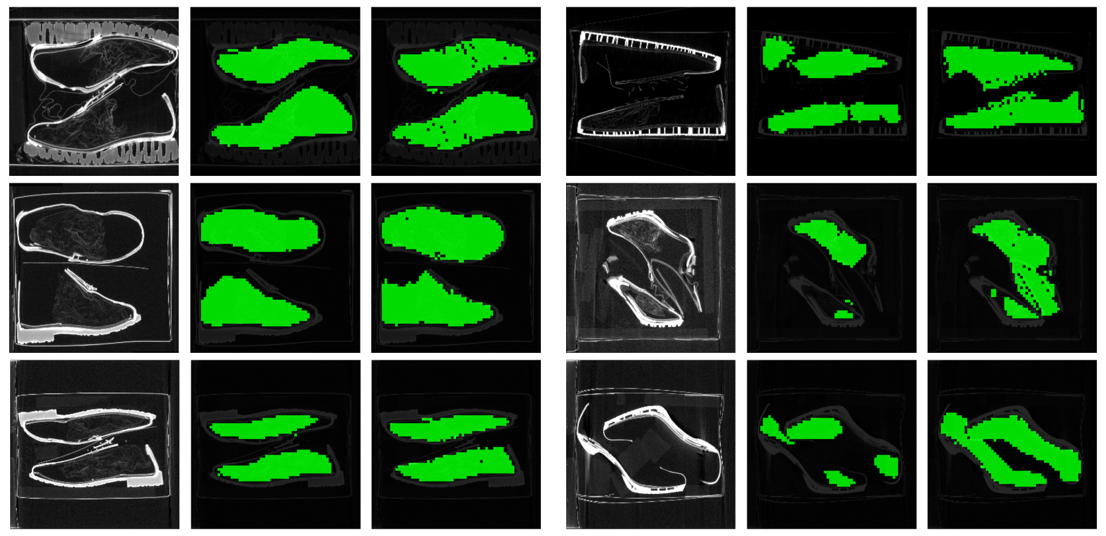
\includegraphics[width=1.0\textwidth]{./images/Paper_2Segments.png}
	
\includegraphics[width=0.9\textwidth]{./images/color_legend_2_classes.png}
	\caption[Results of shoes with 2 segments: background and inside volume]{Results of shoes with 2 segments: background and inside volume. From left to right: the input image, the predicted segmentation, and the corresponding ground truth segmentation image for each of the two columns. The images on the left have high overal F1-score ({\tt \small Shoepassion\_40\_down2\_2\_2: 0.936 [0.983, 0.889]\footnotemark; PetrolioSch-40-float\_down2\_2\_2: 0.919 [0.987, 0.852]; Petrolio-Sch-dunkelbraun\_44\_down2\_2\_2: 0.932 [0.995, 0.871]}), the images on the right have a low F1-score ({\tt \small Adidas\_Martin: 0.777 [0.983, 0.571]; Citywalk-sit-taupe-36\_down2\_2\_2: 0.713 [0.979, 0.447]; Tamaris-Pump-schwarz\_42\_down2\_2\_2: 0.755 [0.991, 0.519]}).}
	\label{Paper_2Segments}
\end{figure}
\footnotetext{{The order of these numbers are: total F1-score of the volume, in brackets the F1-score of background, and inside volume.}}

An analysis of the model's predictions using only two segments (background and inside volume) shows that the overall F1-score is very high. This is mainly due to the model's consistent ability to accurately identify the background, often achieving scores higher than 0.98. In contrast, the segmentation of the inside volume is less precise, leading to a lower F1-score for this class. This discrepancy highlights the challenge of identifying fine-grained features within the shoe, especially when visual cues are weak. The model appears to rely heavily on clear structural boundaries to segment the inside volume effectively. As a result, any ambiguity in shape or texture directly impacts performance. Improving the segmentation of the inside volume may therefore require more diverse training data or enhanced feature representations.

\medskip

A comparison between predictions with high and low scores indicates that the model performs well when the boundary of the sole and the upper material is clearly distinguishable, as can be seen in figure \ref{Paper_2Segments}. In such cases, the inside volume is segmented with high accuracy. However, when the boundary is unclear or contains open areas, as seen in the lower right image, the model often predicts the inside volume only at the tip and heel of the shoe, resulting in a reduced F1-score. This behavior suggests that the model struggles to generalize to less distinct input patterns, particularly in regions with missing or ambiguous boundary information.

\medskip

The results of experiment 3 are shown in table \ref{tab:paper_4_segments} and figure \ref{Paper_4Segments}:
\begin{center}
	\begin{threeparttable}[H]
		\begin{tabular}{lcc}
			\toprule[1.5pt]  
			& \multicolumn{2}{c}{Network} \\
			\multicolumn{1}{l}{F1-score} & {Residual SE UNet} & {SHViT Segformer} \\
			\midrule
			\midrule
			Total          & $0.873$ & $0.702 \pm 0.003$ \\
			\midrule
			Background     & $0.997$ & $0.984 \pm 0.000$ \\
			Outer Sole     & $0.887$ & $0.777 \pm 0.006$ \\
			Inner Sole     & $0.795$ & $0.459 \pm 0.012$ \\
			Upper Material & $0.813$ & $0.586 \pm 0.008$ \\
			\bottomrule
		\end{tabular}
		\captionsetup{width=0.95\textwidth}
		%		\captionsetup{width=\textwidth}
		\caption[Comparison of segmentation performance (F1-scores) between the Residual SE UNet and SHViT Segformer models across four different classes]{Experiment 3: Comparison of segmentation performance (F1-scores) between the Residual SE UNet and SHViT Segformer models across four different classes. The F1-score of UNet model for the segments \enquote{Inner Sole} and \enquote{Upper Material} is higher than for the SHViT Segformer model. Data for Residual SE UNet are taken from Table 4 \cite{contribution_martin_leipert}.}
		\label{tab:paper_4_segments}
	\end{threeparttable}
\end{center}

\begin{figure}[H]
	\centering
	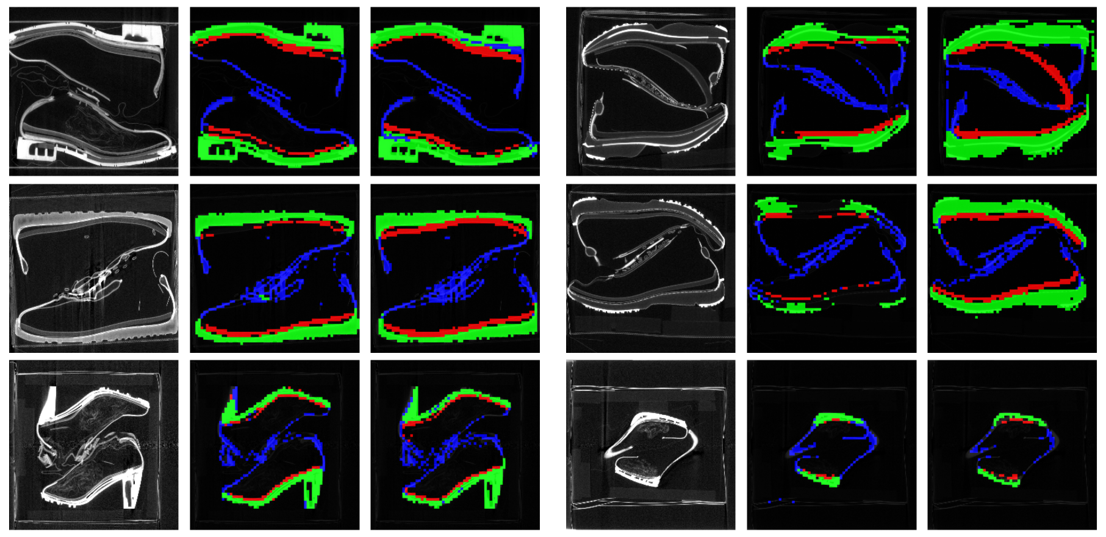
\includegraphics[width=1.0\textwidth]{./images/Paper_4Segments.png}
	
\includegraphics[width=0.8\textwidth]{./images/color_legend_4_classes.png}
	\caption[Results of shoes with 4 segments: background, outer and inner sole, and upper material]{Results of shoes with 4 segments: background, outer sole, inner sole, and upper material. From left to right: the input image, the predicted segmentation, and the corresponding ground truth segmentation image for each of the two columns. The images on the left have high overal F1-score ({\tt \small Bruschi\_down2\_2\_2: 0.764 [0.982, 0.811, 0.605, 0.660]\footnotemark; Camper\_down2\_2\_2: 0.777 [0.971, 0.875, 0.550, 0.711]; Citywalk-sit-taupe-39\_down2\_2\_2: 0.768 [0.994, 0.840, 0.598, 0.641]}), the images on the right have a low F1-score ({\tt \small Puma\_38\_down2\_2\_2: 0.645 [0.940, 0.631, 0.386, 0.624]; Puma\_Silver\_down2\_2\_2:  0.580 [0.948, 0.431, 0.353, 0.589]; Tamaris-Pump-Schwarz-38\_down2\_2\_2: 0.643 [0.995, 0.665, 0.513, 0.400]}).}
	\label{Paper_4Segments}
\end{figure}
\footnotetext{{The order of these numbers are: total F1-score of the volume, in brackets the F1-score of background, outer sole, inner sole, and upper material.}}

Analyzing the standard deviation of the predictions for the 40 shoes reveals the class that is most difficult to predict. In this case, the thin layer of the inner sole shows the highest standard deviation of 0.11, indicating a substantial variation between accurate and less accurate predictions. The outer sole and upper material follow, each with a standard deviation of approximately 0.08. In contrast, the background exhibits a low deviation, indicating more consistent predictions for this class. The green area shown in the two images in the upper right represents the outer sole of the shoe. The model encounters difficulties, visible as unfilled gaps in the image, when the bright line of the outer sole suddenly changes from light to dark. In contrast, no such issues occur when the outer sole is depicted with consistent brightness.

\medskip

It was also observed that the model can produce a visually good prediction while still achieving a low F1-score. This can be seen, for example, in the bottom right image when comparing the predicted image with the ground truth. It is noticeable that in the ground truth image, the upper material (blue color) is not fully represented. Since the F1-score is calculated by comparing the prediction with the ground truth, discrepancies between the two inevitably lead to a lower score, even though the prediction itself is actually of good quality.

\bigskip

The experimental results summarized in tables \ref{tab:paper_3_segments} to \ref{tab:paper_4_segments} show that \gls{shvit} performs not as well as UNet-\gls{cnn}. A literature review offers more details about this performance gap.

\medskip

Convolutional networks like the Residual SE UNet generally outperform transformer-based models such as \gls{shvit} Segformer in semantic segmentation tasks, especially on small datasets. One of the main reasons is that \glspl{cnn} have a strong inductive bias \cite{Dosovitskiy2021ViT}. They are designed to recognize local patterns like edges and textures, which helps them generalize well even from limited data. In contrast, Vision Transformers lack this bias and need much more training data to learn spatial relationships effectively \cite{ronneberger2015, steiner2022trainvitdataaugmentation}.

\medskip

Moreover, \glspl{cnn} like UNet use skip connections that preserve high-resolution features, which is especially important for accurately segmenting small or fine-grained objects (e.g., shoe tongues or packaging material) \cite{zhou2018unet}. Transformers, when trained from scratch, tend to produce coarser outputs and have problems capturing such details. This implies that without large datasets or pretrained weights, \glspl{vit} struggle to capture fine structure, which supports the claim of coarser outputs and weaker detail segmentation. As a result, the UNet model performs more robustly in data-scarce, detail-sensitive segmentation scenarios \cite{steiner2022trainvitdataaugmentation}.


{\subsection[Experiment 4: Standard 3D SHViT Segformer Model Evaluation]{Experiment 4: Standard 3D SHViT Segformer Model \\ Eva\-luation}
The fourth experiment uses a standard \gls{3d} \gls{shvit} model configuration to establish baseline performance metrics for the transformer-based segmentation approach. This experiment provides a reference point for evaluating the effectiveness of the hierarchical vision transformer architecture in the specific application domain.

\begin{center}
	\begin{threeparttable}[H]
		\begin{tabular}{lcc}
			\toprule[1.5pt]  
			& \multicolumn{1}{c}{Network} \\
			\multicolumn{1}{l}{F1-score} & {SHViT Segformer} \\
			\midrule
			\midrule
			Total              & $0.485 \pm 0.009$ \\
			\midrule
			Background         & $0.950 \pm 0.009$ \\
			Box                & $0.442 \pm 0.024$ \\
			Inner Sole         & $0.462 \pm 0.010$ \\
			Outer Sole         & $0.742 \pm 0.009$ \\
			Upper Material     & $0.522 \pm 0.006$ \\
			Tongue/Flap        & $0.156 \pm 0.028$ \\
			Packaging Material & $0.120 \pm 0.013$ \\
			\bottomrule
		\end{tabular}
		\captionsetup{width=0.95\textwidth}
		%		\captionsetup{width=\textwidth}
		\caption[Segmentation performance (F1-scores) of the SHViT Segformer across seven classes]{Experiment 4: Segmentation performance (F1-scores) of the SHViT Segformer across seven classes. Results for the Residual SE UNet are not available for this experimental setup. The model performs well on large structures like \enquote{Background} and \enquote{Outer Sole}, but has problems with fine-grained regions such as \enquote{Packaging Material} and \enquote{Tongue / Flap}.}
		\label{tab:paper_7_segments}
	\end{threeparttable}
\end{center}

Small objects or specific components such as the shoe tongue or packaging material exhibit poor segmentation performance, resulting in significantly low F1-scores for these classes. This poor performance in segmenting fine-detailed or smaller features has a substantial impact on the overall F1-score of the model, as these classes contribute disproportionately to the averaged total score. Results\footnote{The results shown in Figure \ref{result_for_shvit_with_center_attention} were generated using a resolution of {\tt (224,224,224)}, but there is little noticeable difference compared to images with an edge length of 256 pixels.} of can be found in figure \ref{result_for_shvit_with_center_attention} on page \pageref{result_for_shvit_with_center_attention}.

\medskip

It is important to note that the current results were obtained using only 40 pairs of shoes, split for training in a 5-fold cross-validation setup with data augmentation. Given the limited size of the dataset, these results should be considered as a baseline, providing a foundation for further investigations or improvements through larger datasets, refined annotations, or more advanced model architectures.



\section{Recommended Model Configuration}
Based on the investigations conducted and discussed in the preceding sections of this chapter, the following conclusions have been drawn and corresponding recommendations are provided: The model achieving the highest F1-accuracy, along with the most favorable accuracy-to-memory trade-off, is the \gls{3d} \gls{shvit}-SegFormer with central self-attention configured with the B5/S2 parametrization\footnote{see also table \ref{tab:variants} in section \ref{sec:Architecture_of_SHViT_Segformer} on page \pageref{sec:Architecture_of_SHViT_Segformer}} and two convolutional heads in the \gls{shvit} encoder head. The kernel size of the central self-attention layer is 3 due to its F1-score with low deviation. It achieves for an input volume of {\tt (224,224,224)} an F1 of $0.480 \pm 0.005$, with a memory consumption of 8.05\,GB and a training time of around 13 seconds per epoch. With this configuration input volumes up to {\tt (320,320,320)} are possible.
   % (\chapter{})
\cleardoublepage

\chapter{Summary, Conclusions, and Future Work}
\glsresetall
In this thesis, existing \gls{2d} Vision Transformer models, SegFormer with \gls{mvt} and \gls{shvit}, were adapted to handle \gls{3d} volumetric data. These models were specifically utilized to identify seven segments: {\tt Background}, {\tt Karton}, {\tt Außensohle}, {\tt Innensohle}, {\tt Obermaterial}, {\tt Zunge}, and {\tt Füllmaterial} from the \gls{3d} shoe scans. The F1-score was employed as the evaluation metric. To address the problem of memory-intensive attention mechanisms, with a complexity of $O(n^2)$, central self-attention (sliding window) was implemented to enhance performance.

\bigskip

The changes made to SegFormer with \gls{mvt} and \gls{shvit} have effectively facilitated the processing of \gls{3d} volumetric data for complex segmentation tasks, specifically targeting shoe scans. By incorporating central self-attention through a sliding window approach, the typical high memory demands of standard attention mechanisms were substantially reduced. This innovation not only extends the applicability of Vision Transformers but also establishes a foundation for more efficient and scalable solutions within \gls{3d} data environments. This research highlights the potential for implementing advanced model architectures across new domains, offering valuable perspectives on integrating \gls{2d} model principles into \gls{3d} datasets. Future endeavors may focus deeper on optimizing attention mechanisms and expanding experimentation to include various types of \gls{3d} segmented data.

\medskip

A series of experiments were conducted to compare the SegFormer model integrated with different backbones: \gls{mvt}, \gls{shvit}, and \glsxtrshort{shvit_csa} evaluating both F1-score and \glsxtrshort{gpu} memory consumption, along with varied hyperparameter configurations. The experiments revealed the superior performance of \gls{shvit} models over \gls{mvt}, showing comparable F1-scores between \gls{shvit} and the central self-attention equipped model. Nevertheless, the central self-attention model exhibited approximately 45\% lower memory usage compared to the standard \gls{shvit} models.

\medskip

In terms of hyperparameter configurations, \gls{shvit_csa} with two convolutional layers in the PatchEmbed block and B5/S2 configuration emerged as most effective, demonstrating the optimal F1/\glsxtrshort{gpu} memory ratio. This configuration allowed for an increase in maximum volume dimensions up to {\tt (320,320,320)}, while constraint memory usage remained within the 24\,GB limit of the graphics card. Additionally, when adjusting kernel sizes, a kernel size of 1 displayed slightly superior potential relative to the standard variant with a kernel size of 3. The benefit of kernel size 1 lies in its precision in detail focus, whereas kernel size 3 and larger resulted in excessive convolution across the relatively small volume of {\tt (28,28,28)} in the central self-attention block, decreasing efficiency.

\medskip

These advancements not only broaden the functional scope of Vision Transformers but also enhance the efficiency and scalability of solutions within \gls{3d} data environments. The insights gained from this research contribute to the ongoing development of attention mechanisms and model architectures, paving the way for further exploration in diverse \gls{3d} data segmentation applications.

\bigskip

Future research could explore the implementation of additional Vision Transformer models as backbones and compare their performance with \gls{shvit}. Addressing the high memory demand of the attention block remains an area for investigation. New advanced techniques might offer further potential for reducing memory consumption. However, going beyond the currently maximal usable volume of {\tt (320,320,320)} may prove challenging due to the constraints imposed by the 24\,GB limit of the graphics card. For \gls{shvit} models with two convolutional layers in the PatchEmbed block within the \gls{shvit} head, the next larger volume would be {\tt (352,352,352)}, but for sure hard to reach. Therefore, innovative strategies are needed to enable efficient scaling without surpassing hardware limitations.
   % Conclusion (\chapter{Conclusion}  TEXT)
%\cleardoublepage


\appendix
\cleardoublepage
\chapter[Setting up Windows Subsystem for Linux (WSL)]{Setting up Windows Subsystem for Linux (WSL) on Windows 11} \label{sec::WSL}
To facilitate the execution of Linux-based software and tools in a Windows environment, Windows Subsystem for Linux (WSL) was set up on a Windows 11 machine. The following steps outline the process of setting up WSL, installing Miniconda, and creating a virtual environment to run PyTorch 2.60\footnote{The PyTorch version 2.5.1 is also working.} with GPU support.

After downloading and installing Ubuntu 24.04 using Microsoft Store the following steps have to be carried out. Before step 4 is executed Miniconda had to be downloaded\footnote{\url{https://www.anaconda.com/download/success}}:
\begin{tcolorbox}[breakable, enhanced, width=\textwidth, colback={lightgray}]  
\begin{Python}
1  sudo apt update -y
2  sudo apt upgrade -y
3  cd /mnt/c/Users/USERNAME/Downloads/
4  bash Miniconda3-latest-Linux-x86_64.sh
5  cd ~
6  ~/miniconda3/bin/conda init bash
7  ~/miniconda3/bin/conda init zsh
8  exit
\end{Python}
\end{tcolorbox}		

The installation of PyTorch is very easy and does not require additional  CUDA drivers or other dependencies, unlike TensorFlow. PyTorch comes with built-in CUDA support\footnote{\url{https://pytorch.org/get-started/locally/}}, meaning it can be simply installed using {\tt pip}, and it will automatically handle the necessary CUDA libraries.
\begin{tcolorbox}[breakable, enhanced, width=\textwidth, colback={lightgray}]  
\begin{Python}
 9  conda create -n torch260 python=3.12
10  conda activate torch260
11  pip3 install torch torchvision torchaudio --index-url https://download.pytorch.org/whl/cu126
12  conda install -c conda-forge opencv matplotlib tqdm seaborn pandas plotly lightning
13  pip install torchsummary torchviz pydicom slicerio unfoldNd vedo
14  sudo apt-get install graphviz
15  cd /mnt/c/Users/USERNAME/Documents/Python/shoes_segformer/Software/
16  pip install PythonTools-3.7.0-py2.py3-none-any.whl
17  conda install conda-forge::libsqlite --force-reinstall
18  conda install conda-forge::sqlite --force-reinstall
\end{Python}
\end{tcolorbox}		
After setting up PyTorch, essential libraries like {\tt matplotlib}, {\tt tqdm}, {\tt seaborn}, etc.~needed for running the SegFormer scripts have to be installed. Additionally, {\tt pydicom} and {\tt slicerio} were included for handling the annotation files for the shoe files. To extract data from the original shoe volume data from the files in {\tt .rek} dataformat, the {\tt PythonTools} software was required.

While running the scripts in VSCode, the kernel occasionally crashed. This issue was resolved by reinstalling the {\tt sqlite} and {\tt libsqlite} packages at the end\footnote{\url{https://stackoverflow.com/a/79484466/27900239}}.
   % appendix A
\chapter{3D-Segmentation Models in Pytorch} \label{code_implementation}
The following code is a modification of the original implementation \cite{IMvision12}, with adjustments and enhancements made to handle \gls{3d} image data effectively. In the following sections, the modified code for all modules needed to perform image segmentation on \gls{3d} images is shown.

\medskip

The code for \gls{shvit} in section \ref{sec::shvid_3d.py} is based on the original implementation from \cite{github_shvit} and has been slightly modified to function as a standalone version without requiring additional package installations. 

\medskip

Note that in this thesis also code for \gls{2d} image segmentation is used but only the code for \gls{3d} segmentation is shown in the sections below. The \gls{2d} version can be implemented by removing all \gls{3d}-specific parts and replacing them with their \gls{2d} counterparts (i.e.~{\tt Conv3D} by {\tt Conv2D}, or remove code with {\tt D=D} and the lines that use the shape of depth).

\medskip

The full source code used in this thesis is available on GitHub of \gls{fau}: \url{https://git5.cs.fau.de/uw61ehod/shvit_segformer_ba}


\section{Sourcecode for 3D-Segformer models} \label{sec::segformer_main}
The main models are located in the file {\tt segformer\_3d.py}. Here the individual modules for Mix-Vision Transformer, \gls{shvit} and SegformerHead are combined to form the final Segformer models. The source code for the remaining modules is organized into separate program files, with links to the corresponding GitHub repository provided below.


\subsection{{\tt segformer\_3d.py}}
The code implements the 3D segmentation models {\tt SegFormer3D} and {\tt SegFormer3D\_SHViT}. 

\medskip

\noindent Key Components:
\begin{itemize}
	\item {\tt SegFormer3D}: The main segmentation model that integrates {\tt MixVisionTransformer3D}, {\tt SegFormerHead3D}, and {\tt ResizeLayer3D}, and supports different configurations specified in {\tt MODEL\_CONFIGS}.

	\item {\tt SegFormer3D\_SHViT}: The main segmentation model integrates {\tt SHViT3D}, {\tt SegFormerHead3D}, and {\tt ResizeLayer3D}, and supports different configurations specified in {\tt MODEL\_CONFIGS} and {\tt SHVIT\_CONFIG}.
\end{itemize}

The SegFormer model implementation, along with its variants used in this thesis, is available in the project's GitHub repository: \url{https://git5.cs.fau.de/uw61ehod/shvit_segformer_ba/-/blob/main/models_torch/segformer_3d.py}.



\subsection{{\tt attention\_3d.py}}
The \gls{3d} Attention Layer is a neural network module implemented using PyTorch. This layer is designed to handle 3-dimensional input data and apply a self-attention mechanism, which allows the network to focus on different parts of the input for each output. Code is based on \cite{IMvision12}, it was modified for PyTorch implementation and adapted to support 3D segmentation.

\medskip

\noindent Key features of the {\tt Attention3D} Layer:
\begin{itemize}
	\item Multi-head Attention: This helps the model focus on information from different parts of the data at the same time, improving its ability to understand various features of the input.
	
	\item Spatial Reduction: Optionally, the input data can be spatially reduced, which can help in managing large input dimensions and improving computational efficiency.
	
	\item Query, Key, and Value Projections: The layer uses linear projections to create queries, keys, and values from the input data, which are essential components of the attention mechanism.
	
	\item Dropout Mechanism: Dropout is applied both to the attention weights and the final projections to prevent overfitting and to improve the model's generalization abilities.
	
	\item Layer Normalization: When spatial reduction is applied, layer normalization helps in stabilizing and speeding up the training process.
\end{itemize}

The code for the \gls{3d} Attention Layer is available in the project's GitHub repository: \url{https://git5.cs.fau.de/uw61ehod/shvit_segformer_ba/-/blob/main/models_torch/attention_3d.py}.


\subsection{{\tt head\_3d.py}}
The code provides implementations of various neural network modules to handle 3-dimensional data and includes a \gls{mlp} layer, a convolutional module, and a segmentation head based on the SegFormer architecture. Code is based on \cite{IMvision12}, it was modified for PyTorch implementation and adapted to support \gls{3d} segmentation.

\medskip

\noindent Key Components:
\begin{itemize}
	\item {\tt MLP3D} Layer: This module performs a simple linear projection, effectively transforming the input tensor's dimensions.
	
	\item {\tt ConvModule3D}: A \gls{3d} Convolutional module that applies convolution, batch normalization, and ReLU activation to the input tensor.
	
	\item {\tt SegFormerHead3D}: A segmentation head designed for processing \gls{3d} tensors. It uses \gls{mlp} layers to transform features and a convolutional layer to fuse them, followed by dropout and final prediction layers.
\end{itemize}

Implementation details of the modules for processing \gls{3d} data, including an \gls{mlp} layer, a convolutional block, and a SegFormer-based segmentation head, can be found in the project's GitHub repository: \url{https://git5.cs.fau.de/uw61ehod/shvit_segformer_ba/-/blob/main/models_torch/head_3d.py}.



\subsection{{\tt modules\_3d.py}}
The code describes a \gls{3d} Vision Transformer model with various neural network modules, including a depth-wise convolution layer, a multi-layer perceptron (\gls{mlp}) with depth-wise convolution, a transformer block with multi-head self-attention, overlapping patch embedding, and the main transformer model is available at the project's GitHub repository: \url{https://git5.cs.fau.de/uw61ehod/shvit_segformer_ba/-/blob/main/models_torch/modules_3d.py}. The code is based on \cite{IMvision12}, it was modified for PyTorch implementation and adapted to support \gls{3d} segmentation.

\medskip

\noindent Key Components:
\begin{itemize}
	\item {\tt DWConv3D}: A depth-wise convolution layer designed to process \gls{3d} data, applying convolution across each spatial dimension.
	
	\item {\tt Mlp3D}: A multi-layer perceptron that includes linear projections, depth-wise convolution, activation, and dropout mechanisms.
	
	\item {\tt Block3D}: A transformer block that combines multi-head self-attention with an \gls{mlp}, including layer normalization and dropout.
	
	\item {\tt OverlapPatchEmbed3D}: A patch embedding layer that creates overlapping patches from the input \gls{3d} data, transforming spatial dimensions into sequence representations.
	
	\item {\tt MixVisionTransformer3D}: The main transformer model that combines patch embedding and multiple transformer blocks to process \gls{3d} data, enabling the extraction of hierarchical features from the input.
\end{itemize}




\subsection{{\tt utils\_3d.py}} \label{sec::utils_3d.py}
The code defines two utility layers aimed at enhancing the performance and usability of \gls{3d} neural network models in PyTorch. These layers include a layer for resizing \gls{3d} input tensors and another for applying the DropPath regularization technique to improve model generalization. The code is based on \cite{IMvision12}, it was modified for PyTorch implementation and adapted to support \gls{3d} segmentation.

\medskip

\noindent Key Components:
\begin{itemize}
	\item {\tt ResizeLayer3D}: This layer resizes \gls{3d} input tensors to a target depth, height, and width using trilinear interpolation.
	
	\item {\tt DropPath3D}: This layer applies the stochastic depth (DropPath) regularization technique, which randomly drops paths during training to prevent overfitting.
\end{itemize}

The code is accessible via the GitHub repository: \url{https://git5.cs.fau.de/uw61ehod/shvit_segformer_ba/-/blob/main/models_torch/utils_3d.py}.



\subsection{{\tt center\_attention\_3d.py}} \label{sec::center_attention_3d.py}
In the code a local (kernel‑based) central self‑attention over a \gls{3d} volume is implemented. Instead of attending globally to every voxel, it:
\begin{itemize}
	\item Slides a cubic window ($k$ kernel) over the volume. Each query only attends to its local $k^3$ neighborhood (rather than the full volume).
	\item For each center position, computes \gls{q} from that center and \gls{k}/\gls{v} from its local neighborhood.
	\item Performs scaled dot‑product attention within each cube.
	\item Outputs an updated feature for each center voxel.
\end{itemize}
The code is very efficient because it is using {\tt unfold} and batched \gls{q}/\gls{k}\gls{v} to reduce memory compared to a full self‑attention function. The code is based on \cite{Li_2022}, it was modified for PyTorch implementation and adapted to support \gls{3d} segmentation and is available here: \url{https://git5.cs.fau.de/uw61ehod/shvit_segformer_ba/-/blob/main/models_torch/center_attention_3d.py}




\subsection{{\tt shvit\_3d.py}} \label{sec::shvid_3d.py}
The code represents a modified version of a PyTorch module designed for visual processing tasks, such as image classification or detection, utilizing the Vision Transformer architecture. The code is based on \cite{yun2024shvit}, it was modified and adapted to support \gls{3d} segmentation.

\medskip

\noindent Key Components:
\begin{itemize}
	\item {\tt GroupNorm} Class: Implements Group Normalization for input tensors. Normalizes the input tensor across spatial dimensions (height and width).
	
	\item {\tt Conv3d\_BN} Class: Combines a \gls{3d} Convolutional layer followed by Batch Normalization. Includes an optional activation function and the ability to fuse convolution and batch normalization layers.
	
	\item {\tt make\_divisible} Function: Ensures that a value is divisible by a specified divisor, which is useful for network architectures that require certain quantities (like the number of channels) to be divisible by a specific number.
	
	\item {\tt SqueezeExcite3D} Class: Implements the \gls{se} module, which recalibrates input features based on their inter-channel dependencies.
	
	\item {\tt PatchMerging3D} Class: Implements a patch merging mechanism using convolutional layers to reduce the spatial dimensions of the input tensor while increasing the number of channels.
	
	\item {\tt Residual3D} Class: Implements a residual connection for layers, optionally including dropout.
	
	\item {\tt FFN3D} Class: Defines a \gls{ffn} with two {\tt Conv3d\_BN} layers and a {\tt ReLU} activation function between them.
	
	\item {\tt SHSA3D} Class: Defines a \gls{shsa} mechanism for processing partial input dimensions.

	\item {\tt SHCSA3D} Class: Defines the modified \gls{shsa} mechanism with central self-attention for processing partial input dimensions.
	
	\item {\tt BasicBlock3D} Class: Represents a basic block for the \gls{shvit} architecture, combining convolutional layers, self-attention, and feed-forward networks through residuals.
	
	\item {\tt SHViT3D} Class: Incorporates the main \gls{shvit} model with hierarchical stages.
	Contains a patch embedding mechanism and multiple stages, each consisting of blocks that process the input tensor through convolutional, self-attention, and feed-forward layers.
	The forward method processes the input tensor through these stages and returns the output tensors for different stages.
\end{itemize}

This code implements a Vision Transformer model with hierarchical stages, incorporating custom features like Group Normalization, Squeeze-and-Excitation, and Residual connections: \url{https://git5.cs.fau.de/uw61ehod/shvit_segformer_ba/-/blob/main/models_torch/shvit_3d.py}. The goal is to enhance the Vision Transformer's performance by integrating these additional components for improved feature processing and representation.


\subsection{{\tt shoes3D\_torch\_B5\_S2\_SW\_001\_2conv3d\_224x224x224.ipynb}} \label{sec::standard'odell_nb}
The filename follows a structured naming convention that encodes key details about the notebook’s purpose, dataset, model architecture, configuration settings, and input data dimensions. The notebook implements a \gls{3d} convolutional neural network in PyTorch for classifying \gls{3d} voxel representations of shoe models, using the code described in the previous sections \url{https://git5.cs.fau.de/uw61ehod/shvit_segformer_ba/-/blob/main/shoes3D_torch_B5_S2_SW_001_2conv3d_224x224x224.ipynb}.

\begin{itemize}
	\item \textbf{Imports:} Load all necessary libraries, including PyTorch, NumPy, and Matplotlib.
	\item \textbf{Configuration:} Define key training parameters such as {\tt EPOCHS}, {\tt BATCH\_SIZE}, and {\tt LEARNING\_RATE}, and set paths to the training and test datasets.
	\item \textbf{Dataset:} Implement the {\tt Shoe3DDataset} class, a custom PyTorch {\tt Dataset} for loading and preprocessing \gls{3d} .npy files, extracting labels, and applying optional data augmentations.
	\item \textbf{Model:} Definition of \gls{shvit} with central self-attention
	\item \textbf{Callbacks:} Set up training utilities such as warm-up scheduling, csv-logger, early stopping, and model checkpointing.
	\item \textbf{Training:} Train the model using gradient accumulation to support small batch sizes.
	\item \textbf{Visualization:} Plot training and validation losses as well as F1-scores over epochs.
	\item \textbf{Evaluation:} Evaluate the final trained model on the test dataset and report performance metrics.
\end{itemize}


\subsection{Tools}
Several files were used for dataset preparation, visualization, and for generating the plots presented in this thesis:
\begin{itemize}
	\item {\tt 01\_visualize\_and\_extract\_2D.ipynb}: Generates \gls{2d} visualizations of the shoes (figure~\ref{Bruschi_down2_2_2}) and corresponding segmentation masks (figure~\ref{Bruschi_down2_2_2_Segmentation}) \url{https://git5.cs.fau.de/uw61ehod/shvit_segformer_ba/-/blob/main/01_visualize_and_extract_2D.ipynb}. The paths to the shoe scan and annotation files must be adjusted accordingly.
	\item {\tt 01\_visualize\_and\_extract\_3D.ipynb}: Creates the \gls{3d} dataset, including both shoe and segmentation files, for a predefined shape and number of layers \url{https://git5.cs.fau.de/uw61ehod/shvit_segformer_ba/-/blob/main/01_visualize_and_extract_3D.ipynb}. As above, the paths to the shoe scans and annotation files need to be modified.
	\item {\tt 3d-plot.py}: A standalone script to visualize a \gls{3d} rendering of a shoe object (see figure~\ref{Bruschi_down2_2_2_3d}) \url{https://git5.cs.fau.de/uw61ehod/shvit_segformer_ba/-/blob/main/3d-plot.py}.
	\item {\tt plots.ipynb}: A Jupyter notebook used to generate the plots shown in chapter~\ref{Results_and_Discussion} \url{https://git5.cs.fau.de/uw61ehod/shvit_segformer_ba/-/blob/main/experiment_kFold/plots.ipynb}.
	\item {\tt legende.ipynb}: A Jupyter notebook to generate the legend used in images, see figures \ref{result_for_shvit_with_center_attention}, \ref{comparison_segmentations_for_different_volume_sizes}, \ref{Paper_3Segments}, \ref{Paper_2Segments}, \ref{Paper_4Segments} \url{https://git5.cs.fau.de/uw61ehod/shvit_segformer_ba/-/blob/main/legende.ipynb}.
\end{itemize}
   % appendix A
\cleardoublepage
%\include{thesis10}   % appendix B
%\cleardoublepage
%\include{thesis11}   % appendix C
%\cleardoublepage

%% Do not change, auto-generated lists of figures, tables and literature %%
% Glossar
\printunsrtglossary[type=abbreviations]
\cleardoublepage

% List of figures
\addcontentsline{toc}{chapter}{\listfigurename}
\listoffigures
\cleardoublepage

% List of tables
\addcontentsline{toc}{chapter}{\listtablename}
\listoftables
\cleardoublepage

% Literature list
% %CONFIG:
%\selectlanguage{german}{\addcontentsline{toc}{chapter}{\bibname}}
\selectlanguage{english}{\addcontentsline{toc}{chapter}{\bibname}}

\printbibliography

\end{document}

